\documentclass[11pt,openany]{book}

\usepackage[utf8]{inputenc}
\IfFileExists{lmodern.sty}{\usepackage[T1]{fontenc}\usepackage{lmodern}}{}
\usepackage[margin=1.15in]{geometry}
\usepackage{microtype}
\usepackage{amsmath,amssymb,amsthm}
\usepackage{graphicx}
\usepackage{booktabs}
\usepackage{tabularx}
\usepackage{longtable}
\usepackage{listings}
\usepackage{xcolor}
\usepackage{etoolbox}
\usepackage[authoryear,round]{natbib}
\usepackage[hidelinks]{hyperref}
\usepackage{caption}

\graphicspath{{figures/}{results/}}

\theoremstyle{definition}
\newtheorem{definition}{Definition}[chapter]
\newtheorem{hypothesis}{Hypothesis}
\theoremstyle{remark}
\newtheorem{remark}{Remark}[chapter]

\lstset{
  basicstyle=\ttfamily\scriptsize,
  breaklines=true,
  columns=fullflexible,
  frame=single,
  rulecolor=\color{black!30},
  numbers=left,
  numberstyle=\tiny\color{black!50},
  showstringspaces=false,
  upquote=true,
  literate={—}{{-}}1 {→}{{->}}1 {Δ}{{$\Delta$}}1 {│}{{|}}1 {├}{{+}}1 {└}{{+}}1 {─}{{-}}1 {▼}{{v}}1
}

% ------------------------------------------------------------
% Results produced by code/occupation.py. If results/results.tex
% is absent every value prints as [pending].
% ------------------------------------------------------------
\newcommand{\pending}{\textbf{[pending]}}
\InputIfFileExists{results/results.tex}{}{}
\InputIfFileExists{results/extras.tex}{}{}
\providecommand{\xThrottleMin}{\pending}
\providecommand{\xDlgPTen}{\pending}
\providecommand{\xDlgPTwentyFive}{\pending}
\providecommand{\xDlgPSeventyFive}{\pending}
\providecommand{\xDlgPNinety}{\pending}
\providecommand{\xDlgInBlockMedian}{\pending}
\providecommand{\xDlgOutBlockMedian}{\pending}
\providecommand{\xCenterAdvDlg}{\pending}
\providecommand{\xCenterAdvOther}{\pending}
\providecommand{\xOccMedian}{\pending}
\providecommand{\xOccPNinety}{\pending}
\providecommand{\xOccPNinetyNine}{\pending}
\providecommand{\xOccPlateauShare}{\pending}
\providecommand{\xRelMax}{\pending}
\providecommand{\xLevelMax}{\pending}
\providecommand{\xOccSeconds}{\pending}
\providecommand{\xOccInBlocks}{\pending}
\providecommand{\xOccInBlocksShare}{\pending}
\providecommand{\xDialogueBelowIntegrated}{\pending}
\providecommand{\xOtherRawIn}{\pending}
\providecommand{\xOtherRawOut}{\pending}
\providecommand{\xOtherResIn}{\pending}
\providecommand{\xOtherResOut}{\pending}
\providecommand{\xBarrageIn}{\pending}
\providecommand{\xBarrageOut}{\pending}
\providecommand{\xDrumIn}{\pending}
\providecommand{\xDrumOut}{\pending}
\providecommand{\xHarshIn}{\pending}
\providecommand{\xHarshOut}{\pending}
\providecommand{\xSpanStart}{\pending}
\providecommand{\xSpanEnd}{\pending}
\providecommand{\xSpanMin}{\pending}
\providecommand{\xSpanRecoverySeconds}{\pending}
\providecommand{\xSpanExceedShare}{\pending}
\providecommand{\xSpanAtOrBelowShare}{\pending}
\providecommand{\xSpanMedianRel}{\pending}
\providecommand{\xBeforeExceedShare}{\pending}
\providecommand{\xBeforeAtOrBelowShare}{\pending}
\providecommand{\xBeforeInBlockShare}{\pending}
\providecommand{\xSpanInBlockShare}{\pending}
\providecommand{\xSegmentRows}{\multicolumn{6}{c}{\pending}}
\providecommand{\resRun}{no}
\providecommand{\resDialogueRef}{\pending}
\providecommand{\resDialogueFallback}{no}
\providecommand{\resDialogueCenter}{\pending}
\providecommand{\resDialogueSeconds}{\pending}
\providecommand{\resDialogueShare}{\pending}
\providecommand{\resDelta}{10}
\providecommand{\resMergeGap}{5}
\providecommand{\resMinBlock}{60}
\providecommand{\resExceedFive}{\pending}
\providecommand{\resExceedTen}{\pending}
\providecommand{\resExceedFifteen}{\pending}
\providecommand{\resExceedTwenty}{\pending}
\providecommand{\resPNinetyFive}{\pending}
\providecommand{\resPNinetyNine}{\pending}
\providecommand{\resOccBlocksN}{\pending}
\providecommand{\resOccTotalMin}{\pending}
\providecommand{\resOccLongestMin}{\pending}
\providecommand{\resOccLongestStart}{\pending}
\providecommand{\resThrottleMedian}{\pending}
\providecommand{\resThrottleMax}{\pending}
\providecommand{\resBarrageBlocksN}{\pending}
\providecommand{\resBarrageLongestMin}{\pending}
\providecommand{\resRecoveryGapLongestMin}{\pending}
\providecommand{\resRecoveryGapLongestStart}{\pending}
\providecommand{\resSwellN}{\pending}
\providecommand{\resSwellFromQuiet}{\pending}
\providecommand{\resSwellIntoOcc}{\pending}
\providecommand{\resSwellLarge}{\pending}
\providecommand{\resAbsRecoveryN}{\pending}
\providecommand{\resAbsRecoveryShare}{\pending}
\providecommand{\resAbsGapLongestMin}{\pending}
\providecommand{\resAbsGapLongestStart}{\pending}
\providecommand{\resDebtMax}{\pending}
\providecommand{\resOmegaIn}{\pending}
\providecommand{\resOmegaOut}{\pending}
\providecommand{\resOmegaThreeShare}{\pending}
\providecommand{\resOmegaThreeShareIn}{\pending}
\providecommand{\resAbsGapRows}{\multicolumn{3}{c}{\pending}}
\providecommand{\resLevelUnit}{LUFS}
\providecommand{\resLevelMeasure}{\pending}
\providecommand{\resLoudnessRun}{no}
\providecommand{\resIntegrated}{\pending}
\providecommand{\resLRA}{\pending}
\providecommand{\resLRALow}{\pending}
\providecommand{\resLRAHigh}{\pending}
\providecommand{\resSubRun}{no}
\providecommand{\resSubCues}{\pending}
\providecommand{\resSubSpeechCues}{\pending}
\providecommand{\resSubNonspeechCues}{\pending}
\providecommand{\resSubOffset}{\pending}
\providecommand{\resSubSeconds}{\pending}
\providecommand{\resSubCorrZero}{\pending}
\providecommand{\resSubCorrOffset}{\pending}
\providecommand{\resDialogueRefSub}{\pending}
\providecommand{\resDialogueRefSubCapped}{\pending}
\providecommand{\resDialogueRefProxy}{\pending}
\providecommand{\resProxySeconds}{\pending}
\providecommand{\resProxyPrecision}{\pending}
\providecommand{\resProxyRecall}{\pending}
\providecommand{\resDialogueSource}{\pending}
\providecommand{\resSubInBlocks}{\pending}
\providecommand{\resSubInBlocksShare}{\pending}
\providecommand{\resSwellQuietLevel}{\pending}
\providecommand{\resOmegaResIn}{\pending}
\providecommand{\resOmegaResOut}{\pending}
\providecommand{\resOmegaResThreeShare}{\pending}
\providecommand{\resOmegaResThreeShareIn}{\pending}
\providecommand{\resOccRows}{\multicolumn{7}{c}{\pending}}
\providecommand{\resGapRows}{\multicolumn{3}{c}{\pending}}

\newcommand{\ifresults}[2]{\ifdefstring{\resRun}{yes}{#1}{#2}}

\newcommand{\optfig}[3]{%
  \begin{figure}[htbp]\centering
  \IfFileExists{#1}{\includegraphics[width=#2\linewidth]{#1}}%
    {\fbox{\parbox{0.8\linewidth}{\centering\small\vspace{2em}%
     Figure generated by \texttt{code/occupation.py}\\ (\texttt{#1}) \pending\vspace{2em}}}}
  \caption{#3}\end{figure}}

\title{\textbf{Acoustic Occupation}\\[0.6em]
\Large Salience, Recovery, and the Temporal Organization of Film Sound}
\author{Flyxion\\ \small Independent Researcher}
\date{September 2026\\[1em]\small Working manuscript}

\begin{document}

\frontmatter
\maketitle

\chapter*{Abstract}
\addcontentsline{toc}{chapter}{Abstract}
Complaints about the sound of contemporary films are usually framed as complaints about loudness. This monograph argues that the variable doing the damage is not level but occupation: the proportion and continuity of time during which a soundtrack stays well above the level at which its dialogue is intelligible, together with the scarcity of intervals in which the listener is allowed to recover. The argument is developed through a single worked case, the 2026 action feature \emph{Drive Through Fire}, reproduced on a small bass instrument amplifier from a computer headphone output, where the listener repeatedly reduced the volume to zero for one to two minutes at a time during gunfire and fight sequences. Measured against its own subtitled dialogue with BS.1770 loudness, the film spends almost a third of its audible running time at least 10~dB above dialogue level, on a plateau rather than in extreme peaks, and contains a twenty-minute stretch in which the soundtrack returns to dialogue level for only half a minute; standard loudness figures for the same film show none of this. The monograph presents the measurement pipeline built to analyse that soundtrack, documents in detail the ways its first versions failed, introduces a dialogue-referenced definition of occupation that avoids the circularity of percentile thresholds, and specifies a response measure (logged volume throttling) and an intervention (a dialogue-forward downmix) that together turn a single listening report into a falsifiable research programme. Claims are graded throughout as established, measured in this study, hypothesised, or rejected.

\chapter*{Preface}
\addcontentsline{toc}{chapter}{Preface}
This study began with a practical failure of listening. A feature film was playing through a small bass practice amplifier connected to the headphone socket of a computer, and for long stretches the only workable response to its soundtrack was to turn the volume all the way down and wait for the scene to end. Dialogue, when it returned, was too quiet to follow at the setting that had made the preceding gunfire tolerable. The volume went up for speech and down again for action, over and over, and some action sequences outlasted any patience for riding the control.

That experience is the only direct observation of listener behaviour in the monograph, and it is treated accordingly. It is reported once, in Chapter~\ref{ch:case}, as the report of a single listener on a single viewing through an unmeasured playback chain. Everything else in the book either measures the soundtrack itself, describes the instruments used to do so, or specifies what would have to be collected for the report to become evidence rather than motivation.

The book is organised as a sequence of instruments and their limits. Part~I states the problem and the conceptual framework. Part~II describes the analysis pipeline and, at some length, the ways its earlier versions produced confident nonsense: a swell detector that was an inverted transient detector, harshness scores that peaked in digital silence, and summary statistics whose values were fixed in advance by the thresholds that produced them. These failures are kept in the text because they are instructive and because a reader deserves to know how the current numbers were reached. Part~III applies the corrected instruments to the case. Part~IV specifies a response measure and an intervention, both of which were first sketched as speculative tools in July 2025 and are here developed into a research design. Part~V grades what has and has not been shown.

Numerical results that depend on the dialogue-referenced analysis of Chapter~\ref{ch:framework} are generated by \texttt{code/occupation.py} and \texttt{code/occupation-extras.py} and inserted automatically. \ifresults{In this build they have been generated from the analysis tables of the film.}{In this build they have not yet been generated, and each such value prints as \pending. Appendix~\ref{app:repro} gives the commands that fill them in.}

The code, the figures, and the manuscript source are released into the public domain.


\tableofcontents

\mainmatter

\part{The Problem}
\chapter{Occupation, Not Loudness}
\label{ch:intro}

\section{A familiar complaint, stated precisely}

Few complaints about home viewing are as common as the one about dialogue and explosions. The volume that makes speech intelligible makes the action unbearable; the volume that makes the action tolerable makes the speech inaudible. Viewers respond by keeping a hand on the remote. Industry responses have been largely framed in terms of loudness: broadcast loudness normalisation, legislation against loud advertisements, and dynamic range compression modes built into consumer decoders. These responses treat the problem as one of level.

This monograph takes a different view. The difficulty is not that a soundtrack is loud, nor even that it has a wide dynamic range. Both are ordinary properties of cinema sound, and both are intended. The difficulty arises from three conditions holding together:
\begin{enumerate}
\item the listening level is set for dialogue, because dialogue is what must be understood;
\item non-dialogue material exceeds that level by a large margin; and
\item it does so for long, nearly continuous stretches, with few intervals in which the level returns to the dialogue range.
\end{enumerate}
The first condition fixes a reference. The second is a question of magnitude. The third is a question of temporal organisation, and it is the one that loudness measures summarise away. An integrated loudness figure for a film is a single number over its whole running time; a loudness range figure describes a distribution. Neither says whether the loud material arrives as occasional peaks separated by long rests or as a continuous block several minutes long. The distinction between those two cases is the subject of this book.

\section{Peak intensity and occupation}

The central distinction can be stated compactly. \emph{Peak intensity} concerns how far above the reference a soundtrack goes. \emph{Occupation} concerns how much of the time it stays there, and how continuously. A conventional dramatic structure has a rhythm of rest, rise, peak, and release. A soundtrack can instead proceed through rise, impact, barrage, further rise, and further impact without returning to rest. The second pattern need not have higher peaks than the first. What distinguishes it is that the listener is never released.

The practical consequence is that the listener's volume control becomes part of the soundtrack's reproduction. If the reference is set for speech and the soundtrack occupies the range well above it for minutes at a time, the listener must either accept the exceedance, reduce the volume and lose the next line of dialogue, or reduce the volume to nothing and wait. The case at the centre of this study involved the last of these. For action sequences lasting one to two minutes or more, the volume was turned fully down until the scene calmed.

\section{Why a single case}

This monograph is built around one film, \emph{Drive Through Fire}, and one reproduction setup. That is a limitation and it is stated as such. It is also a methodological choice. The concepts needed to describe the problem (dialogue reference, exceedance, occupation block, recovery window, salience channel, throttle) are not yet standard, and the instruments needed to measure them do not exist off the shelf. A single case examined closely is the right scale at which to build and debug those instruments. The case is not offered as evidence that contemporary film mixing is generally at fault. It is offered as a worked example of how that question could be answered.

\section{Grading claims}

Every substantive claim in the book is assigned one of four grades, and Chapter~\ref{ch:conclusion} tabulates them.

\begin{description}
\item[Established.] Claims supported by standards, published measurement, or well-replicated psychoacoustics, independent of this study. Example: cinema reproduction is calibrated to a reference sound pressure level; home reproduction generally is not.
\item[Measured.] Claims about the \emph{Drive Through Fire} soundtrack that follow from the analysis pipeline as corrected, with the caveats of Chapters~\ref{ch:pipeline} and~\ref{ch:failures}.
\item[Hypothesised.] Claims that the framework predicts and that the measurements are consistent with, but that require listener data, a comparison corpus, or measurement of the playback chain to test.
\item[Rejected.] Claims that were made during the analysis, sometimes confidently, and that did not survive inspection. These are kept because the errors are instructive.
\end{description}

\section{Plan of the book}

Chapter~\ref{ch:background} surveys the standards and literatures that bear on the problem: loudness measurement, cinema calibration, film sound practice and theory, psychoacoustics, and noise annoyance. Chapter~\ref{ch:framework} gives formal definitions and states the hypotheses. Chapter~\ref{ch:pipeline} describes the analysis pipeline. Chapter~\ref{ch:failures} documents its failures and their corrections. Chapter~\ref{ch:chain} treats the reproduction chain as an object of study in its own right. Chapter~\ref{ch:case} presents the case. Chapter~\ref{ch:overdetermination} examines the co-occurrence of salience channels. Chapter~\ref{ch:response} specifies the response measure and the study design needed to test the framework against listener behaviour. Chapter~\ref{ch:intervention} develops an intervention. Chapter~\ref{ch:conclusion} grades the results.

\chapter{Background: Standards, Practice, and Perception}
\label{ch:background}

This chapter gathers the material the framework depends on. It is not a survey of film sound studies. It collects, from several fields that rarely cite each other, the pieces needed to state the problem of occupation precisely: how loudness is measured and regulated, how cinema reproduction is calibrated and why home reproduction differs, how film sound is organised in practice, and what psychoacoustics and noise research say about intelligibility, annoyance, and recovery.

\section{Measuring loudness}

The reference algorithm for programme loudness is ITU-R BS.1770 \citep{itu1770}. It applies a frequency weighting (the K-weighting, a high-shelf and high-pass pair approximating the head's acoustic effect and reduced low-frequency sensitivity), computes mean-square power per channel, sums channels with weights that favour the surrounds slightly, and gates out quiet blocks so that silence does not dilute the result. Its output is expressed in LUFS (or LKFS, the same unit under a different name). European broadcast practice under EBU R\,128 normalises programmes to $-23$~LUFS integrated loudness \citep{ebu128}; North American practice under ATSC A/85 uses $-24$~LKFS \citep{atsc85}. In the United States the Commercial Advertisement Loudness Mitigation Act made A/85 compliance for advertisements a legal requirement \citep{calm2010}.

Integrated loudness is a single number for a whole programme. EBU Tech~3342 supplements it with Loudness Range (LRA), a statistic of the distribution of short-term loudness values after gating, computed as the spread between the 10th and 95th percentiles \citep{ebu3342}. LRA answers how widely the loudness varies. It does not answer how that variation is arranged in time. A programme alternating every ten seconds between quiet and loud passages and a programme with one quiet hour followed by one loud hour can have the same integrated loudness and the same LRA. For the purposes of this study that is the decisive limitation of the standard measures: they are distributional, and occupation is a temporal property.

\section{Dialogue as reference}

Broadcast and home formats already acknowledge that dialogue is the natural anchor for listening level. The AC-3 bitstream carries a \emph{dialnorm} parameter describing the average level of dialogue in the programme, which decoders use to bring dialogue to a common reproduction level; the same format carries dynamic range control profiles that compress loud and quiet passages toward that anchor when the listener selects a reduced-range mode \citep{atsc52}. Consumer ``night mode'' settings are descendants of this mechanism. Their existence is itself evidence, of an institutional kind, that the gap between dialogue level and effects level is a recognised home-listening problem rather than an idiosyncratic one.

Speech intelligibility has its own measurement tradition. The Speech Intelligibility Index \citep{ansi1997} weights frequency bands by their importance to understanding; the most heavily weighted bands lie in the region from roughly one to four kilohertz, where consonant cues are carried. A reproduction chain weak in that region reduces intelligibility at a given level, which in turn raises the level a listener must choose to follow speech. This point returns in Chapter~\ref{ch:chain}.

\section{Cinema calibration and the home}

Theatrical reproduction is calibrated. Under SMPTE practice each screen channel is aligned so that a pink-noise signal at a specified digital reference level produces a specified sound pressure level at the reference listening position, conventionally 85~dB(C) for $-20$~dBFS \citep{smpte200}. Mixing stages are aligned the same way. A film mix is therefore authored for a known relationship between digital level and acoustic level. Its dynamic range, including the distance between dialogue and the loudest effects, is chosen with that relationship in mind.

Home reproduction has no such alignment. The listener chooses the level, typically lower than theatrical reference, and chooses it by ear, usually for dialogue. Equal-loudness relationships are level dependent \citep{fastl2007}, so a mix balanced at reference level is heard with a different spectral balance at lower levels. More importantly for this study, the listener sets the anchor, and the anchor is speech. Everything the mix places far above speech arrives far above the listener's chosen level. A dynamic range that is intended in a calibrated theatre becomes, in an uncalibrated room, a sequence of exceedances that the listener manages by hand.\footnote{This is an established fact about calibration practice, not a claim that any particular film was mixed badly. A mix can be entirely correct for its intended room and still be difficult in an uncalibrated one. The monograph distinguishes these throughout.}

\section{Film sound practice and theory}

The film sound literature of the digital era documents the expansion of dynamic range and low-frequency capacity that multichannel formats made available \citep{sergi2004,kerins2011}. The low-frequency effects channel and the headroom of digital formats allow effects to be much louder, relative to dialogue, than optical soundtracks permitted.

Two ideas from practitioners and theorists are central here. The first is Chion's observation that cinema is \emph{vococentric}: its sound is organised around the voice, and the ordinary work of mixing is to keep speech intelligible against everything else \citep{chion1994}. The complaint at the root of this study is, in Chion's terms, a failure of vococentrism at the point of reproduction. The second is Murch's account of density \citep{murch2005}. Murch describes a practical limit on how many simultaneous layers of sound of the same kind an audience can follow as distinct, and a strategy of distributing layers across contrasting kinds (dialogue, music, effects of different spectral and rhythmic character) so that density does not collapse into undifferentiated mass. Murch's concern is clarity within a moment. The present study's concern is continuity across moments. The two are complementary: a mix can be clear in every individual moment and still occupy the listener for too long.

\section{Psychoacoustics}

Classical psychoacoustics offers measures closer to perception than digital level. Fastl and Zwicker's models of loudness (in sones), sharpness (weighting of high-frequency energy), roughness (fast amplitude modulation), and fluctuation strength (slow modulation), and the psychoacoustic annoyance index built from them, are the standard descriptive vocabulary \citep{fastl2007}. The analysis pipeline of Chapter~\ref{ch:pipeline} uses cruder spectral descriptors (centroid, flatness, zero-crossing rate), and Chapter~\ref{ch:failures} shows one consequence of that choice. Replacing them with the psychoacoustic measures is part of the programme proposed in Chapter~\ref{ch:response}.

Two further psychoacoustic facts matter. Forward masking reduces sensitivity to quiet sounds for a short interval following a loud one \citep{moore2012}, so speech arriving immediately after an impact is harder to hear than the same speech after silence. And the auditory system organises sound into streams by onset, spectrum, and continuity \citep{bregman1990}; abrupt onsets are strong cues for the formation of a new stream and draw attention. A soundtrack dense with abrupt onsets is, in stream terms, repeatedly asking for attention.

\section{Noise, annoyance, and control}

Community noise research establishes that annoyance grows with level, with the number of events, and with their duration \citep{kryter1985,miedema2001}. The finding most relevant here is older and experimental. Glass and Singer showed that the aftereffects of noise exposure on subsequent task performance depended strongly on predictability and on perceived control: participants who believed they could stop the noise showed markedly reduced aftereffects even when they did not use the control \citep{glass1972}. A volume control is exactly such a means of control. Its use during a film is therefore not only a response to excessive sound but a measurable act of regaining control over it, which is part of why Chapter~\ref{ch:response} treats volume behaviour as the natural dependent variable.

\section{Sound, affect, and the soundscape}

Two broader literatures frame the problem. Goodman's account of sonic warfare treats low frequencies and sudden sound as instruments of affective control that operate below deliberate attention \citep{goodman2010}. Schafer's distinction between hi-fi soundscapes, in which discrete sounds are heard clearly against a quiet ground, and lo-fi soundscapes, in which signals crowd each other and perspective is lost, gives a vocabulary for what a highly occupied soundtrack does to a listening room \citep{schafer1977}. Finally, the music-industry ``loudness war'' shows how competitive pressure can push a production norm toward sustained high level at the expense of contrast \citep{vickers2010}. Whether an analogous pressure operates in film mixing is outside this study's evidence, but the analogy explains why the question is worth asking.

\section{The gap}

None of these literatures measures the quantity this study is concerned with: the temporal structure of a soundtrack's exceedances over its own dialogue level, and the behaviour that structure forces on a listener reproducing it at an uncalibrated level through a particular chain. Loudness standards measure distributions. Film theory describes intentions and effects. Psychoacoustics and noise research describe perception and annoyance under controlled conditions. The framework in the next chapter is an attempt to connect them.

\chapter{A Framework for Occupation}
\label{ch:framework}

This chapter defines the quantities used in the rest of the book and states the hypotheses they are meant to test. The definitions are deliberately simple. Each is chosen so that it can be computed from a soundtrack file with the pipeline of Chapter~\ref{ch:pipeline} and so that its dependence on free parameters is explicit.

\section{Time base and level}

Let the film occupy the interval $[0, T]$ and let time be discretised into one-second bins indexed by $t$. Let $L(t)$ denote the level of the reproduced signal in bin $t$, computed as the energy mean of the level values falling in that bin:
\begin{equation}
L(t) = 10\log_{10}\Big(\frac{1}{|F_t|}\sum_{f\in F_t} 10^{\ell_f/10}\Big),
\end{equation}
where $F_t$ is the set of level measurements falling in bin $t$ and $\ell_f$ is the level of measurement $f$. Averaging in the power domain rather than in decibels matters: a second containing one loud impact and otherwise near silence should register the impact, not the silence.

The primary level measure is BS.1770 momentary loudness \citep{itu1770}, measured on the full 5.1 mix at ten values per second and energy-averaged into one-second bins, in LUFS. It applies the standard's K-weighting and channel weights and, as the standard specifies, excludes the low-frequency effects channel. When the film itself is not available to the analysis, the pipeline falls back to unweighted RMS of a mono downmix of the main channels, in dBFS (Chapter~\ref{ch:pipeline}). Only differences in level enter the framework, so the choice of unit does not affect the definitions below, but K-weighting does change which material counts as loud: it discounts low frequencies and emphasises the presence region, closer to how loudness is perceived.

A bin is \emph{audible} if $L(t)$ exceeds a floor $L_{\min}$ (default $-60$~LUFS, or $-65$~dBFS for the RMS fallback). Inaudible bins are excluded from all statistics that are normalised by duration.

\section{The dialogue reference}

Two definitions of dialogue time are used. The primary one is taken from the film's subtitles, which record when speech occurs. The secondary one is a centre-channel proxy, which requires nothing but the audio; it is retained because most films in a comparison corpus will have it and not all will have reliable subtitles, and because comparing it with the subtitle definition measures how far the proxy can be trusted.

\begin{definition}[Subtitled dialogue bins]
Let a subtitle file contain cues $(a_i, b_i, x_i)$ with start and end times and text. Remove cues whose text describes sound rather than speech: text consisting only of bracketed or parenthesised descriptions such as \texttt{[GUNFIRE]} or \texttt{(sighs)}, or of music symbols. Let $\kappa(t)$ be the fraction of bin $t$ covered by the remaining cues after shifting all cue times by an offset $\omega_s$. The set of subtitled dialogue bins is
\begin{equation}
\mathcal{S} = \{\, t : t \text{ audible},\ \kappa(t) \ge 0.5 \,\}.
\end{equation}
\end{definition}

The offset $\omega_s$ corrects for subtitles timed to a different release of the film. It may be given, or estimated as the lag, within $\pm30$~s, that maximises the correlation between cue coverage and centre-channel dominance.

\begin{definition}[Dialogue-likely bins]
Let $C(t)$ and $N(t)$ be the levels of the centre channel and of the non-centre mix (front and surround pairs) in bin $t$. The set of dialogue-likely bins is
\begin{equation}
\mathcal{D} = \{\, t : t \text{ audible},\ C(t) - N(t) \ge c,\ \tau(t) \le Q_{p}(\tau \mid C - N \ge c) \,\},
\end{equation}
where $c$ is a centre-advantage threshold (default 6~dB), $\tau(t)$ is transient activity (Section~\ref{sec:channels}), and $Q_p$ is its $p$-th percentile (default 75) among centre-dominant audible bins.
\end{definition}

The definition encodes a convention of film mixing, that dialogue is carried predominantly in the centre channel, and removes the most transient-heavy centre-dominant bins because centre-panned impacts and gunfire are common in action scenes. It remains a proxy. Music, effects, and ambience can sit in the centre, and dialogue can be spread. Its agreement with $\mathcal{S}$ is reported as precision $|\mathcal{D}\cap\mathcal{S}|/|\mathcal{D}|$ and recall $|\mathcal{D}\cap\mathcal{S}|/|\mathcal{S}|$.

\begin{definition}[Dialogue reference]
The dialogue reference is $D = \operatorname{median}\{L(t) : t\in\mathcal{S}\}$ when subtitles are available, and $D = \operatorname{median}\{L(t) : t\in\mathcal{D}\}$ otherwise.
\end{definition}

Subtitles mark when speech occurs, not how loud it is, and they mark shouted lines inside gunfights as readily as quiet conversation. The median is robust to such lines because most dialogue in most films is not delivered over gunfire. As a check, the reference is also computed with the most transient-heavy quarter of subtitled bins removed.

$D$ is the level at which a listener who sets the volume for speech is anchored. It is internal to the film, and that is intentional: the listener's anchor is also internal to the film.

\section{Exceedance and occupation}

\begin{definition}[Exceedance]
$E(t) = L(t) - D$.
\end{definition}

\begin{definition}[Occupation]
For a tolerance $\delta > 0$ (default 10~dB), bin $t$ is \emph{occupied} if $E(t) \ge \delta$. The occupation fraction is
\begin{equation}
\phi_\delta = \frac{|\{t \text{ audible} : E(t)\ge\delta\}|}{|\{t \text{ audible}\}|}.
\end{equation}
\end{definition}

\begin{definition}[Occupation block]
Let $O$ be the set of occupied bins. Form maximal runs of consecutive bins in $O$, then merge any two runs separated by a gap of at most $g$ seconds (default 5). An \emph{occupation block} is a merged run of total length at least $m$ seconds (default 60).
\end{definition}

The merging step reflects the fact that a two-second dip below $D+\delta$ in the middle of a firefight does not give the listener a usable opportunity to restore the volume. The minimum length $m$ reflects the case: the behaviour at issue is reducing the volume for a minute or more.

A block need not be occupied throughout. Its internal composition is summarised by the share of occupied bins and by percentiles of $E$ within it.

\section{Recovery}

The pipeline of Chapter~\ref{ch:pipeline} defines recovery relatively, as intervals of at least five seconds in which a composite burden score lies in its own bottom quartile. Chapter~\ref{ch:failures} explains why that definition cannot support claims about how much recovery a film provides: roughly a quarter of the film is below its own lower quartile by construction. A relative definition can still locate the longest stretches without recovery, and it is used for that purpose only.

An absolute definition, anchored to the dialogue reference, is preferred:

\begin{definition}[Recovery window]
For a margin $\rho$ and width $w$, a recovery window is an interval of at least $w$ consecutive audible bins in which $E(t)\le\rho$ throughout. The default is $\rho = 0$, $w=5$: at least five seconds at or below dialogue level.
\end{definition}

\begin{definition}[Recovery gap and recovery debt]
A recovery gap is the interval between the end of one recovery window and the start of the next. Within a gap beginning at $t_0$, the recovery debt at time $t$ is
\begin{equation}
K(t) = \sum_{s=t_0}^{t} \max\big(0,\ E(s) - \delta\big).
\end{equation}
\end{definition}

$K$ is a crude accumulator: it grows only while the soundtrack exceeds tolerance and resets only when the soundtrack returns to dialogue level for long enough. It is proposed as a predictor, not a model of physiology.

\section{Salience channels}
\label{sec:channels}

Level is one way a soundtrack claims attention. The pipeline measures four others, each a candidate channel of salience:

\begin{description}
\item[Transient activity $\tau(t)$.] Density of broadband spectral-flux onsets over a five-second window, weighted by audibility.
\item[Low-frequency onset activity $\lambda(t)$.] Density of onsets in the band below 250~Hz over a four-second window. This is often percussion but also engines, impacts, and explosions; it is named for what it measures.
\item[Swell events $\sigma$.] Sustained rises in level of at least 6~dB over windows of two to eight seconds that are not carried by a single step.
\item[Spectral harshness $\eta(t)$.] A composite of spectral centroid, flatness, and zero-crossing rate, weighted by audibility.
\end{description}

\begin{definition}[Overdetermination index]
Given thresholds $\theta_k$ for each channel, $\Omega(t) = \sum_k \mathbf{1}[\,\text{channel } k \text{ elevated at } t\,]$, with level exceedance $E(t)\ge\delta$ counted as one of the channels.
\end{definition}

$\Omega$ counts how many independent means the soundtrack is using at once to claim attention. The name reflects the hypothesis that high $\Omega$ is redundant signalling, several mechanisms communicating the same instruction to attend.

\section{A listener model}

Let the listener set the volume so that dialogue is reproduced comfortably, and let $G(t)\le 0$ be the additional gain applied by the listener at time $t$ relative to that setting. Suppose the listener tolerates reproduced level up to $D+\delta$. Holding a block at tolerance requires $G(t) \le -\max(0, E(t)-\delta)$. Since listeners do not adjust gain second by second, a single setting per block is more realistic. The \emph{implied throttle depth} of a block $b$ is
\begin{equation}
T_b = \max\big(0,\ Q_{95}(E \mid b) - \delta\big),
\end{equation}
the attenuation needed to hold the block's 95th-percentile exceedance at tolerance.

Two responses are available when $T_b$ is large. The listener can attenuate by $T_b$ and lose the dialogue inside the block, which sits at $D + G < D - T_b$, or can turn the volume fully down and wait. The model predicts the second response when $T_b$ is large and the block is long, because attenuation by a large $T_b$ leaves nothing intelligible to attend to anyway. This is the behaviour reported in the case.

\section{Hypotheses}

\begin{hypothesis}[Occupation over level]
Volume reductions are better predicted by occupation variables (current $E(t)$ together with time already spent in the current block) than by instantaneous level alone, and far better than by whole-programme statistics such as integrated loudness or loudness range.
\end{hypothesis}

\begin{hypothesis}[Recovery debt]
Conditional on $E(t)$, the probability of a volume reduction increases with $K(t)$.
\end{hypothesis}

\begin{hypothesis}[Overdetermination]
Conditional on $E(t)$, the probability of a volume reduction increases with $\Omega(t)$.
\end{hypothesis}

\begin{hypothesis}[Chain amplification]
A reproduction chain that is weak in the speech-importance band and that saturates on transients increases effective exceedance: it raises the level needed for intelligible dialogue and adds distortion products during the loudest passages.
\end{hypothesis}

\begin{hypothesis}[Intervention]
A dialogue-forward downmix with dynamic range compression reduces the number and duration of volume reductions without reducing comprehension of the dialogue.
\end{hypothesis}

None of these is tested in this monograph. Chapter~\ref{ch:case} measures the soundtrack-side quantities they depend on. Chapter~\ref{ch:response} specifies the data needed to test them.


\part{Instruments}
\chapter{The Analysis Pipeline}
\label{ch:pipeline}

The quantities of Chapter~\ref{ch:framework} are computed in two stages. The first, \texttt{analyze-soundtrack-v3.1.py}, decodes the film, extracts frame-level features in bounded memory, derives detector scores and events, and writes audition clips. The second, \texttt{occupation.py}, measures BS.1770 loudness in its own decode pass, aligns the film's subtitles, aggregates everything to one-second bins, and computes the dialogue-referenced quantities. Both are listed in Appendix~\ref{app:code}. This chapter describes what they compute and why, and records the parameters that the results depend on.

\section{Design constraints}

A feature film at 48~kHz with six channels is roughly 1.5 billion samples. The first attempt at this analysis computed a short-time Fourier transform of the whole film in memory and was terminated by the operating system. Every later version follows three rules. Decoding and channel manipulation are done by \texttt{ffmpeg}, which streams. Python reads the decoded analysis stems in chunks of sixty seconds and keeps only compact per-frame features. Normalisation statistics are computed only after all chunks have been processed, so that a quiet minute and a loud minute are compared against the same film-wide scale rather than each being treated as its own acoustic universe.

\section{Analysis stems}

Four single-channel stems are produced:

\begin{description}
\item[Broadband.] A mono downmix of the full mix at 16~kHz.
\item[Low band.] The same downmix low-pass filtered at 250~Hz, at 8~kHz.
\item[Centre.] The front centre channel alone, at 16~kHz.
\item[Non-centre.] An equal-weight mix of the front left and right and the two surround channels, at 16~kHz.
\end{description}

One property of the downmix matters for interpretation. When a stream is tagged with a 5.1 layout, the default \texttt{ffmpeg} downmix to mono does not include the low-frequency effects channel. This was verified directly: a test file with a 50~Hz tone in the LFE channel alone produced output at $-91$~dB, while the same tone in the centre channel produced output at $-19.7$~dB. Consequently the ``low-frequency'' measures in this study describe bass carried in the main channels, not the LFE channel. Many software players make the same omission when downmixing for stereo output, so the analysed signal may resemble what a listener on a stereo or mono chain actually hears more closely than a full-range measurement would; this is an assumption to be checked against the player used, not a finding.

\section{Frame features}

Features are computed with \texttt{librosa} \citep{mcfee2015} at a hop of 512 samples (32~ms at 16~kHz):

\begin{description}
\item[Level.] Frame RMS in dBFS.
\item[Onset strength.] Spectral flux on a mel spectrogram in the log domain, the standard onset detection function \citep{bello2005}.
\item[Spectral shape.] Centroid, flatness \citep{johnston1988}, and zero-crossing rate.
\item[Low-band level and onset strength] on the low stem.
\item[Centre and non-centre level.]
\end{description}

Onset strength, centroid, flatness, and zero-crossing rate are all nearly independent of absolute level. A click at $-70$~dBFS produces the same log-domain spectral flux as the same click at $-30$~dBFS; the noise floor of a near-silent passage has maximal flatness. This property is the source of the most consequential failure described in Chapter~\ref{ch:failures}.

\section{Audibility weighting}

Version 3.1 multiplies every shape and transient feature by an audibility weight
\begin{equation}
w(t) = \operatorname{clip}\!\left(\frac{L(t) - L_{\min}}{L_{\text{full}} - L_{\min}},\ 0,\ 1\right),
\end{equation}
with $L_{\min}=-65$ and $L_{\text{full}}=-45$~dBFS by default, and a corresponding weight on the low band with bounds $-70$ and $-50$~dBFS. Robust statistics (median and scaled median absolute deviation, with interquartile and standard-deviation fallbacks when the MAD is degenerate) are computed over audible frames only.

\section{Detectors}

\begin{description}
\item[Impact.] Peaks of a weighted sum of standardised onset, level, and spectral shape, above the 98.5th percentile and at least 0.75~s apart.
\item[Low-frequency onset activity.] Four-second moving density of positive standardised low-band onset strength, combined with low-band level; peaks above the 97.5th percentile at least 4~s apart.
\item[Harshness.] Weighted sum of standardised centroid, flatness, zero-crossing rate, and level; peaks above the 98th percentile at least 3~s apart.
\item[Barrage.] Five-second moving density of positive standardised onset strength, combined with level and centroid; contiguous regions above the 85th percentile lasting at least 3~s.
\item[Burden.] A bounded composite of normalised level, onset strength, low-frequency onset density, centroid, flatness, and barrage density, smoothed over half a second. High-load regions are those above its 80th percentile for at least 4~s; relative recovery regions are those below its 25th percentile for at least 5~s.
\item[Swell.] An event detector described in Chapter~\ref{ch:failures}.
\end{description}

Every detector threshold except the swell detector is a percentile of the film's own score distribution. The consequences of that choice for interpretation are taken up in Chapter~\ref{ch:failures}. The dialogue-referenced quantities of Chapter~\ref{ch:framework} were introduced to avoid them.

\section{Audition clips}

For each of the swell, low-frequency, impact, harshness, and barrage detectors, the twenty highest-scoring candidates are cut from the source as short stereo MP3 clips, with a playlist per category and an annotation table with blank label and notes columns. Point events are cut from twelve seconds before to eight seconds after; swells from four seconds before the rise to six seconds after it; regions from five seconds before their start. This is the bridge from acoustic proxies to identified sources, and Chapter~\ref{ch:response} describes how it must be modified before its labels can count as evidence.

\section{Loudness}

The level measure of Chapter~\ref{ch:framework} is taken from \texttt{ffmpeg}'s \texttt{ebur128} filter, an implementation of BS.1770 and EBU R\,128, run once over the film's full 5.1 stream. The filter reports momentary loudness (400~ms window) ten times a second; these values are energy-averaged into one-second bins. The same pass yields the film's integrated loudness and its loudness range under EBU Tech~3342, which Chapter~\ref{ch:case} sets beside the occupation measures. Both are cached so that later runs do not decode the film again.

The RMS level of the version~3.1 frame table remains available and is used when the film is not supplied. The two measures differ in weighting, channel treatment, and window, and they are not interchangeable in absolute terms; within one analysis only one is used.

\section{Subtitles}

The film's subtitle file (SubRip format) is parsed into timed cues. Formatting tags are stripped and HTML entities decoded. Cues whose text is entirely descriptive of sound, such as \texttt{[GUNFIRE]}, \texttt{(sighs)}, or music symbols, are removed, since subtitles for deaf and hard-of-hearing viewers use them to describe non-speech sound; cues that mix a description with speech, or carry a speaker label before speech, are kept. Each second receives the fraction of its duration covered by remaining cues.

Subtitle files are often timed to a different release of a film, shifted by a few seconds. The script estimates a constant offset by computing the correlation between cue coverage and a binary indicator of centre-channel dominance at lags from $-30$ to $+30$~s in half-second steps, and applies the best lag only if it improves the correlation by more than ten percent over no shift. A fixed offset can be supplied instead. Timing that drifts over the film, as when a subtitle file was made for a version at a different frame rate, is not corrected by a constant offset; the reported correlation at the chosen lag is a check on this.

\section{Parameters}

Table~\ref{tab:params} records the defaults. Every result reported in Chapter~\ref{ch:case} uses them unless stated otherwise.

\begin{table}[htbp]\centering\small
\begin{tabularx}{\linewidth}{lXl}
\toprule
Parameter & Role & Default \\
\midrule
Chunk & Decode and feature window & 60 s \\
Sample rate & Broadband, centre, non-centre stems & 16 kHz \\
Hop & Frame spacing & 512 samples \\
$L_{\min}$, $L_{\text{full}}$ & Audibility weight bounds (frame features) & $-65$, $-45$ dBFS \\
Audibility floor & Per-second bins, BS.1770 level & $-60$ LUFS \\
Low-band bounds & Low-band audibility weight & $-70$, $-50$ dBFS \\
Swell windows & Rise windows & 2, 4, 6, 8 s \\
Swell minimum rise & & 6 dB \\
Subtitle coverage & Minimum cue coverage for a subtitled bin & 0.5 \\
Subtitle offset search & Lag range and step & $\pm30$ s, 0.5 s \\
$c$ & Centre advantage for dialogue-likely bins & 6 dB \\
$p$ & Transient cap percentile for dialogue-likely bins & 75 \\
$\delta$ & Occupation tolerance & 10 dB \\
$g$ & Block merge gap & 5 s \\
$m$ & Minimum reported block & 60 s \\
$\rho$, $w$ & Absolute recovery margin and width & 0 dB, 5 s \\
Channel threshold & Elevated salience channel & 1.5 (standardised) \\
Residual margin & Share of threshold left after level fit & 0.5 \\
\bottomrule
\end{tabularx}
\caption{Pipeline parameters.}\label{tab:params}
\end{table}

\chapter{How the Detectors Failed}
\label{ch:failures}

This chapter documents four failures of the analysis as it was first built and first read. Each produced output that looked meaningful. Each was caught only by comparing one plot against another or by running the pipeline on a synthetic signal whose contents were known. They are recorded in detail because they are generic: any analysis that standardises heavy-tailed features, uses level-invariant descriptors, or thresholds by percentiles is exposed to them.

\section{The swell detector that detected transients}

Version~3 attempted to detect gradual swells by smoothing the level trace, taking its positive gradient, standardising the result by median and median absolute deviation, smoothing again, and subtracting a penalty proportional to positive standardised onset strength so that abrupt impacts would not count as swells.

On the film, more than half of the positive-gradient values were exactly zero, because at any moment the smoothed level is as likely to be falling as rising and every falling frame is clipped to zero. The median was therefore zero and so was the median absolute deviation. The standardisation function returned an array of zeros when the scale was degenerate. The gradient term vanished, and what remained was
\begin{equation}
\text{swell}(t) = -0.25\,\max\big(0,\ z_{\text{onset}}(t)\big),
\end{equation}
an inverted, scaled copy of the onset trace. Figure~\ref{fig:swellfail} shows the result. The deepest troughs of the ``swell'' plot, near $-14$ at about 14 and 63 minutes, sit exactly under the two largest onset peaks. Every swell candidate reported by version~3 was a peak of this inverted function, which is to say a place where nothing happened.

\begin{figure}[htbp]\centering
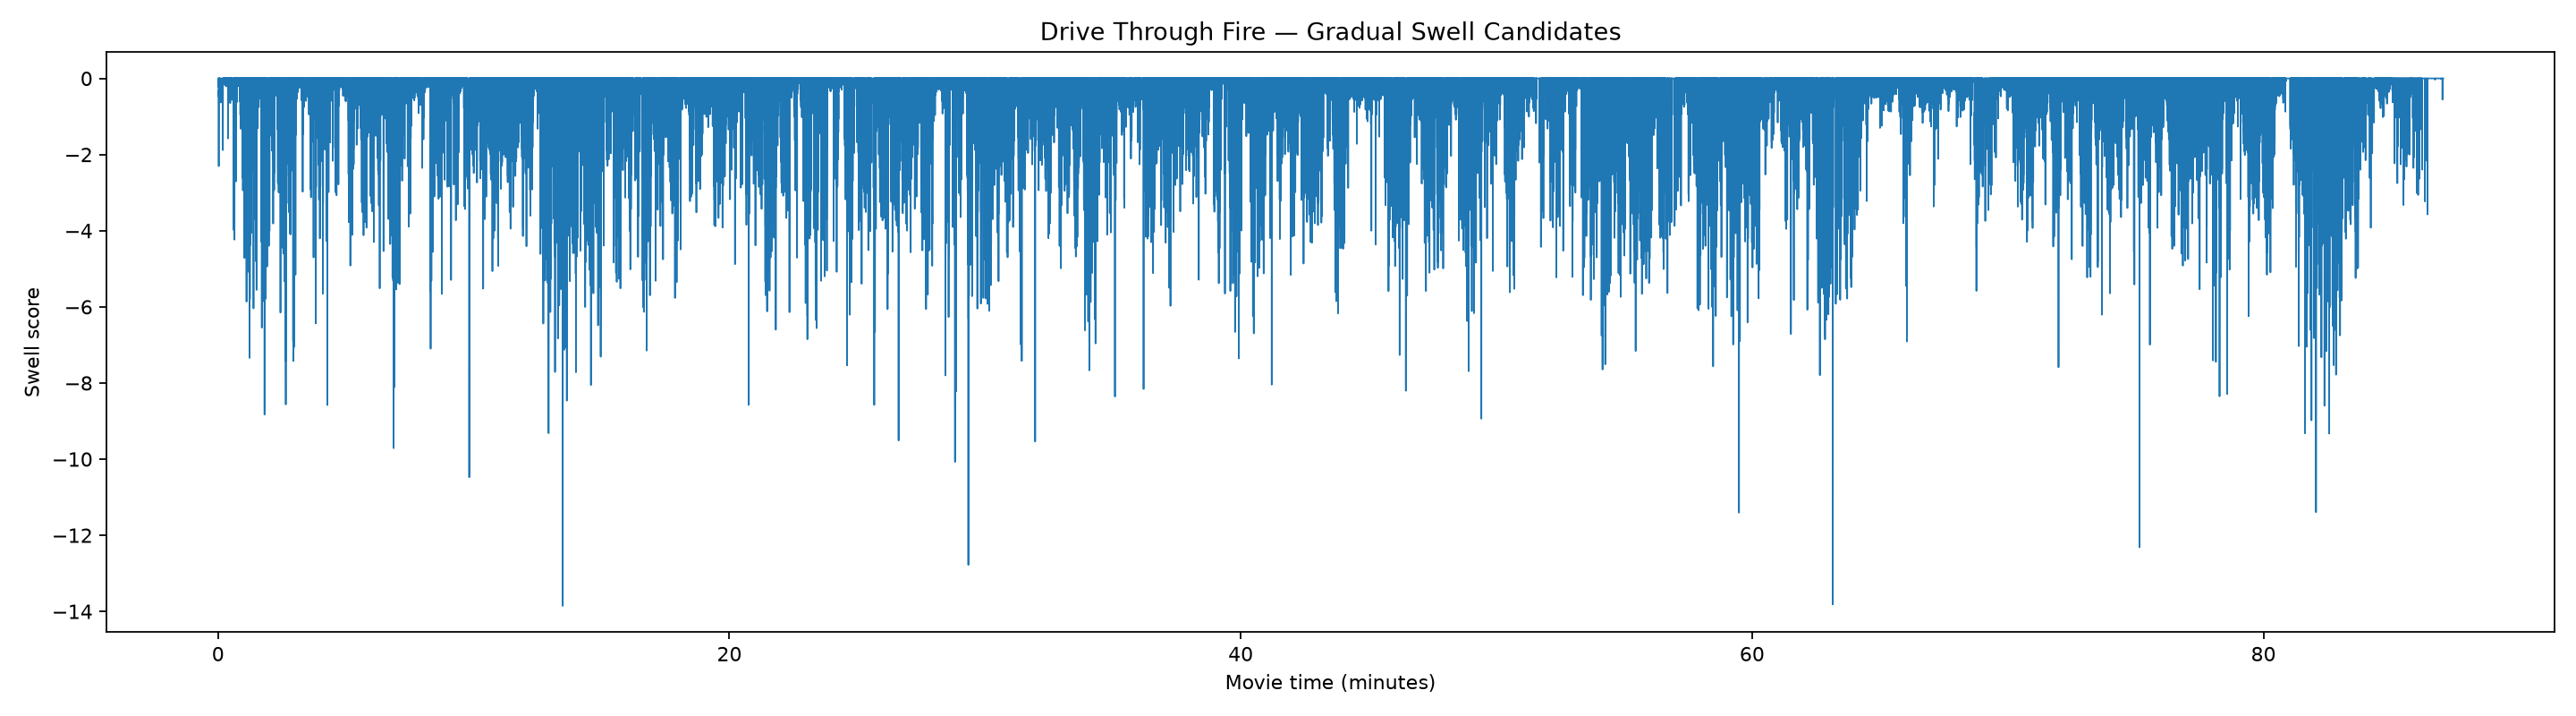
\includegraphics[width=\linewidth]{v3-04-swells.png}\\[0.5em]
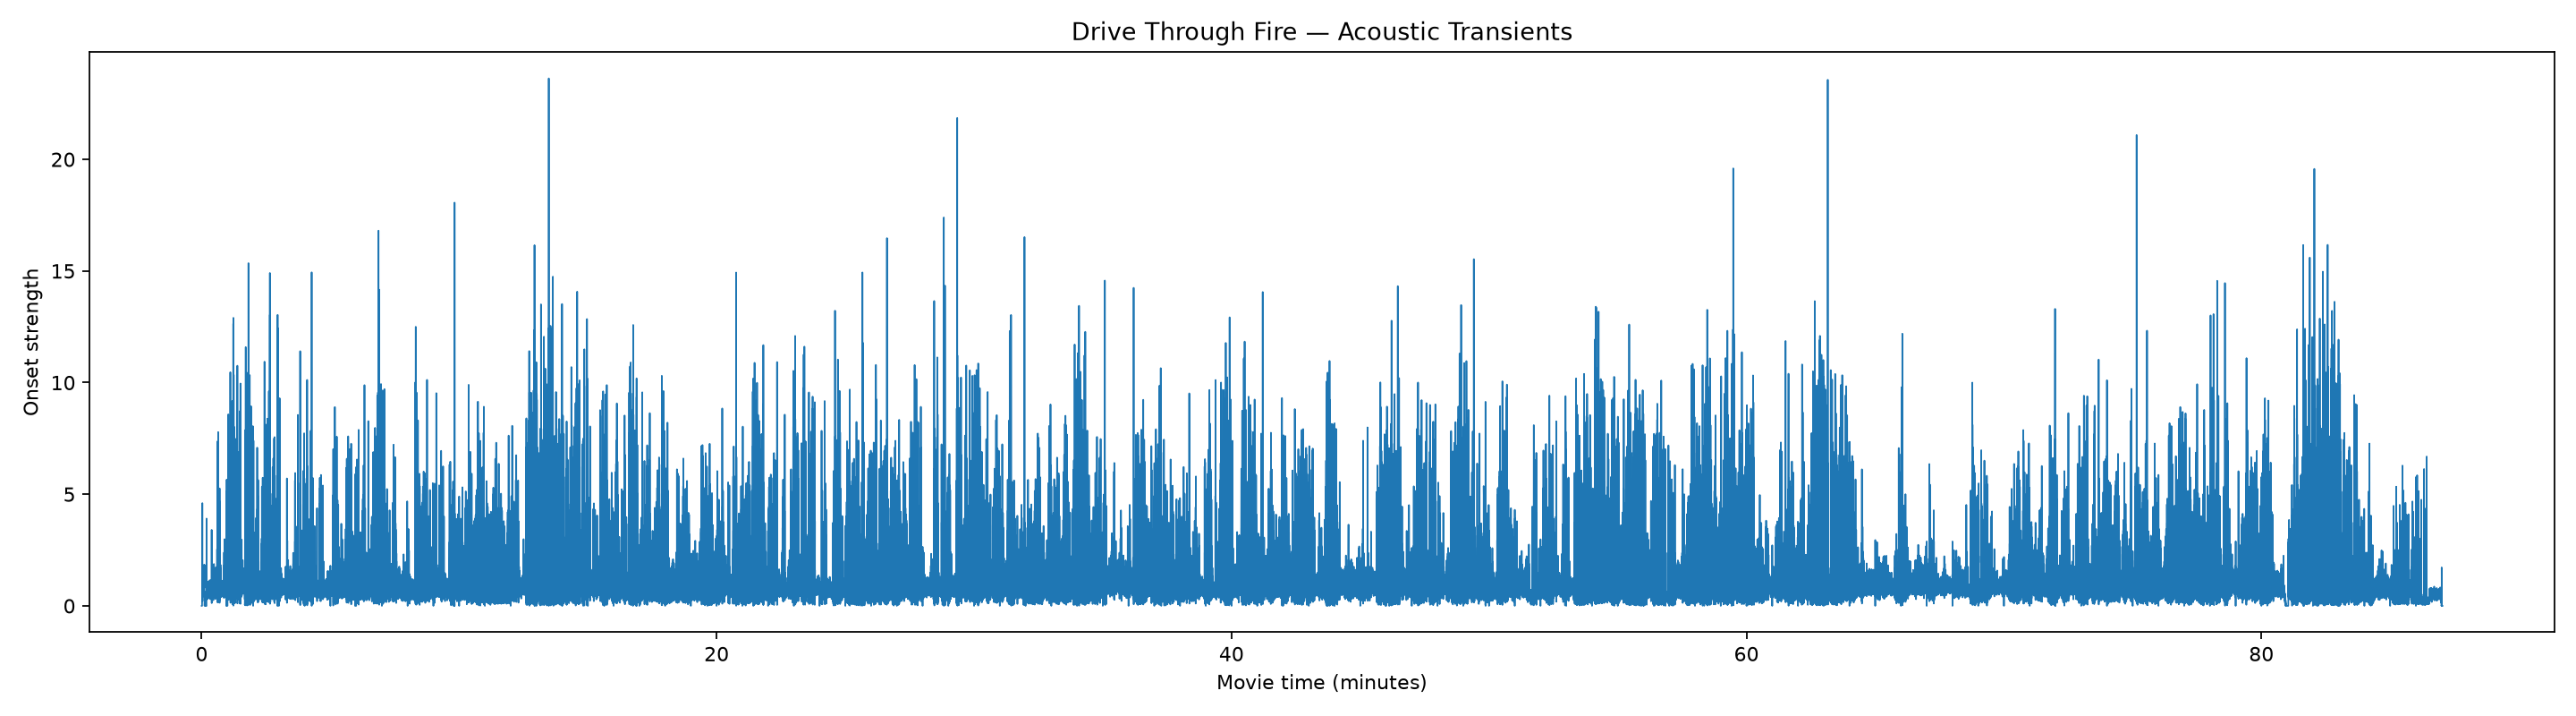
\includegraphics[width=\linewidth]{v3-02-transients.png}
\caption{Version~3 swell score (top) and onset strength (bottom). With a zero MAD the swell score reduced to a negated multiple of positive standardised onset strength; its troughs mirror the onset peaks.}
\label{fig:swellfail}
\end{figure}

The failure is data dependent. On a synthetic test file the same code did not degenerate, because the synthetic signal had fewer exact ties. A test that passes on synthetic data does not certify the code on real data, and the converse also holds; both are needed.

Version~3.1 replaces the frame-level gradient with an event detector. Level is averaged in the power domain over 0.25-second bins and median-filtered over about one second, so that a single transient cannot carry a bin. For each candidate window $\Delta\in\{2,4,6,8\}$ seconds the rise $S(t,\Delta) = L(t+\Delta)-L(t)$ is computed. A candidate is accepted if the rise is at least 6~dB, at least 60\% of the bin-to-bin steps within the window are upward, the two largest steps together account for no more than half the rise, and the window ends above the audibility floor. The two-largest-steps rule was added after a synthetic test showed that a hard cut from near silence into a loud passage, smeared by the analysis window across two bins, otherwise passed as a swell. On the synthetic file the corrected detector recovered a ramp placed between 150 and 158 seconds as an event from 149.25 to 157.25 seconds and reported nothing else.

The standardisation function was also changed so that a degenerate MAD falls back to the interquartile range and then to the standard deviation, rather than silently returning zeros.

\section{Harshness in silence}

The version~3 harshness score combined standardised spectral centroid, flatness, zero-crossing rate, and level. Its largest values in the entire film, near 66 against a typical ceiling around 30, occur at the very start, at about 81 minutes, and at the very end (Figure~\ref{fig:harshfail}). Each coincides with a dropout to digital silence at $-100$~dBFS on the level plot. In near silence the spectrum is the noise floor, which is spectrally flat and dominated by high-frequency dither; flatness and zero-crossing rate are maximal and the centroid is high. The most ``harsh'' moments of the film were the moments with no sound in them.

\begin{figure}[htbp]\centering
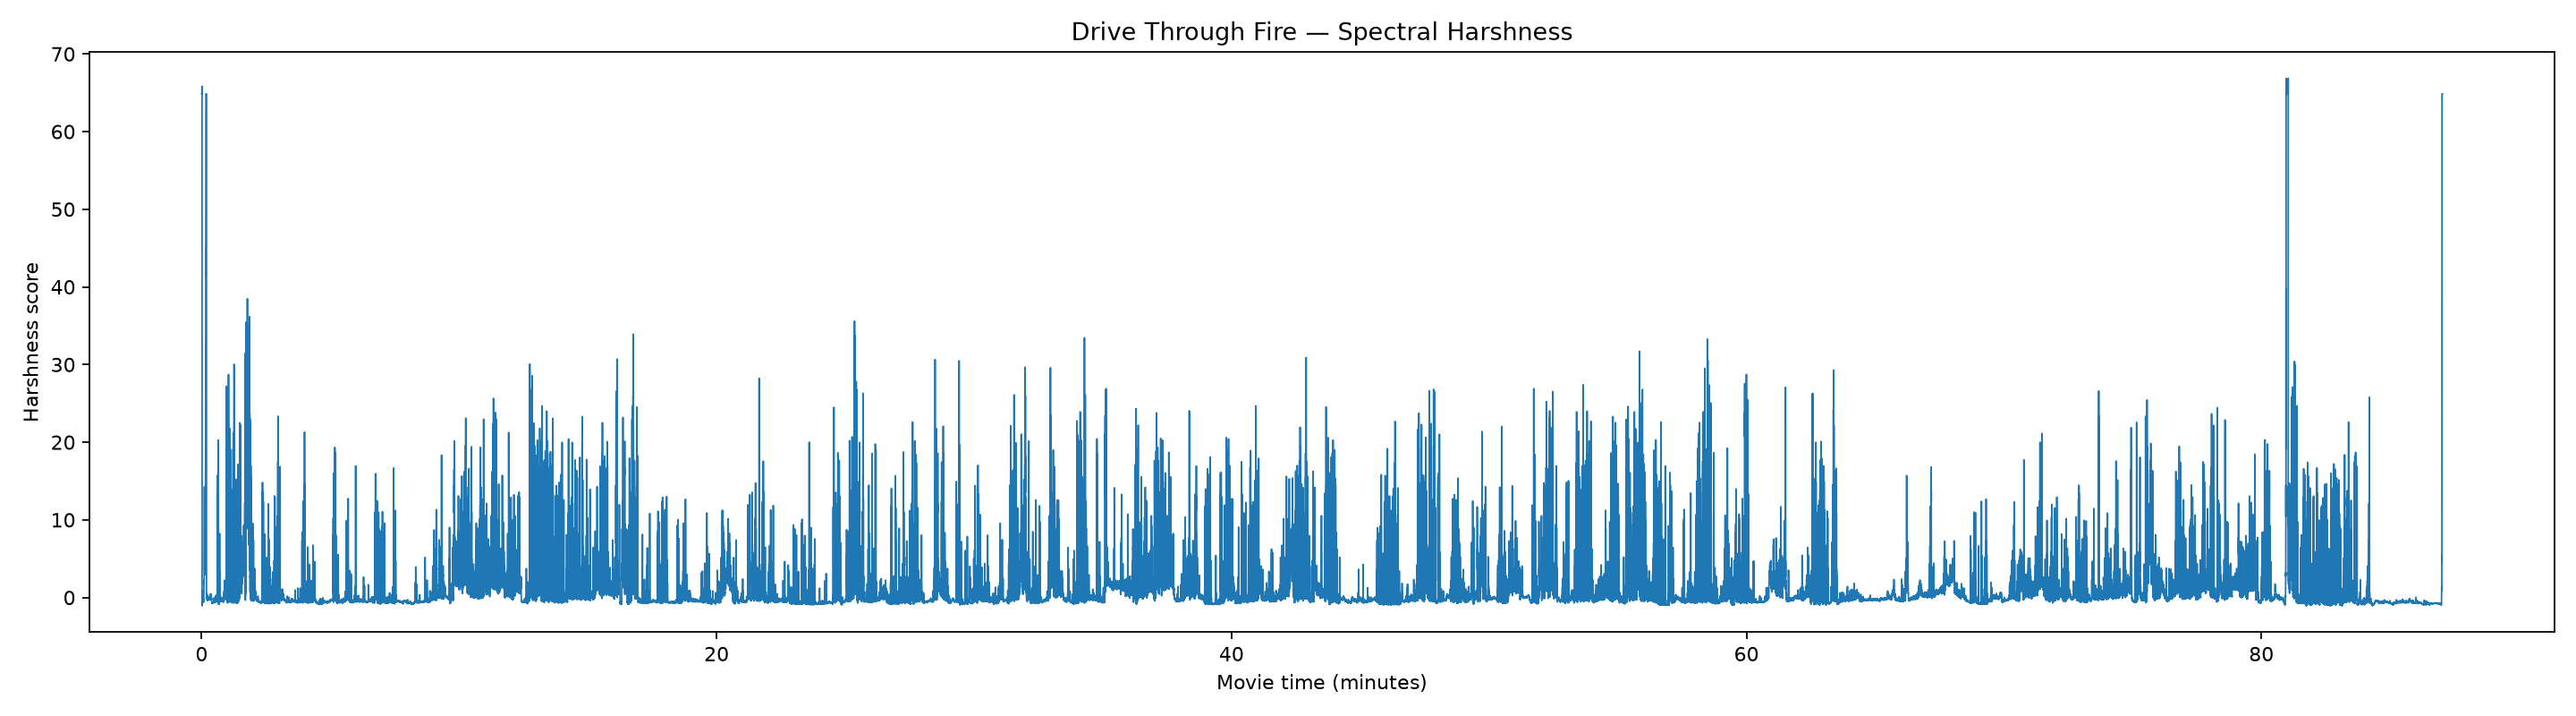
\includegraphics[width=\linewidth]{v3-06-harshness.png}\\[0.5em]
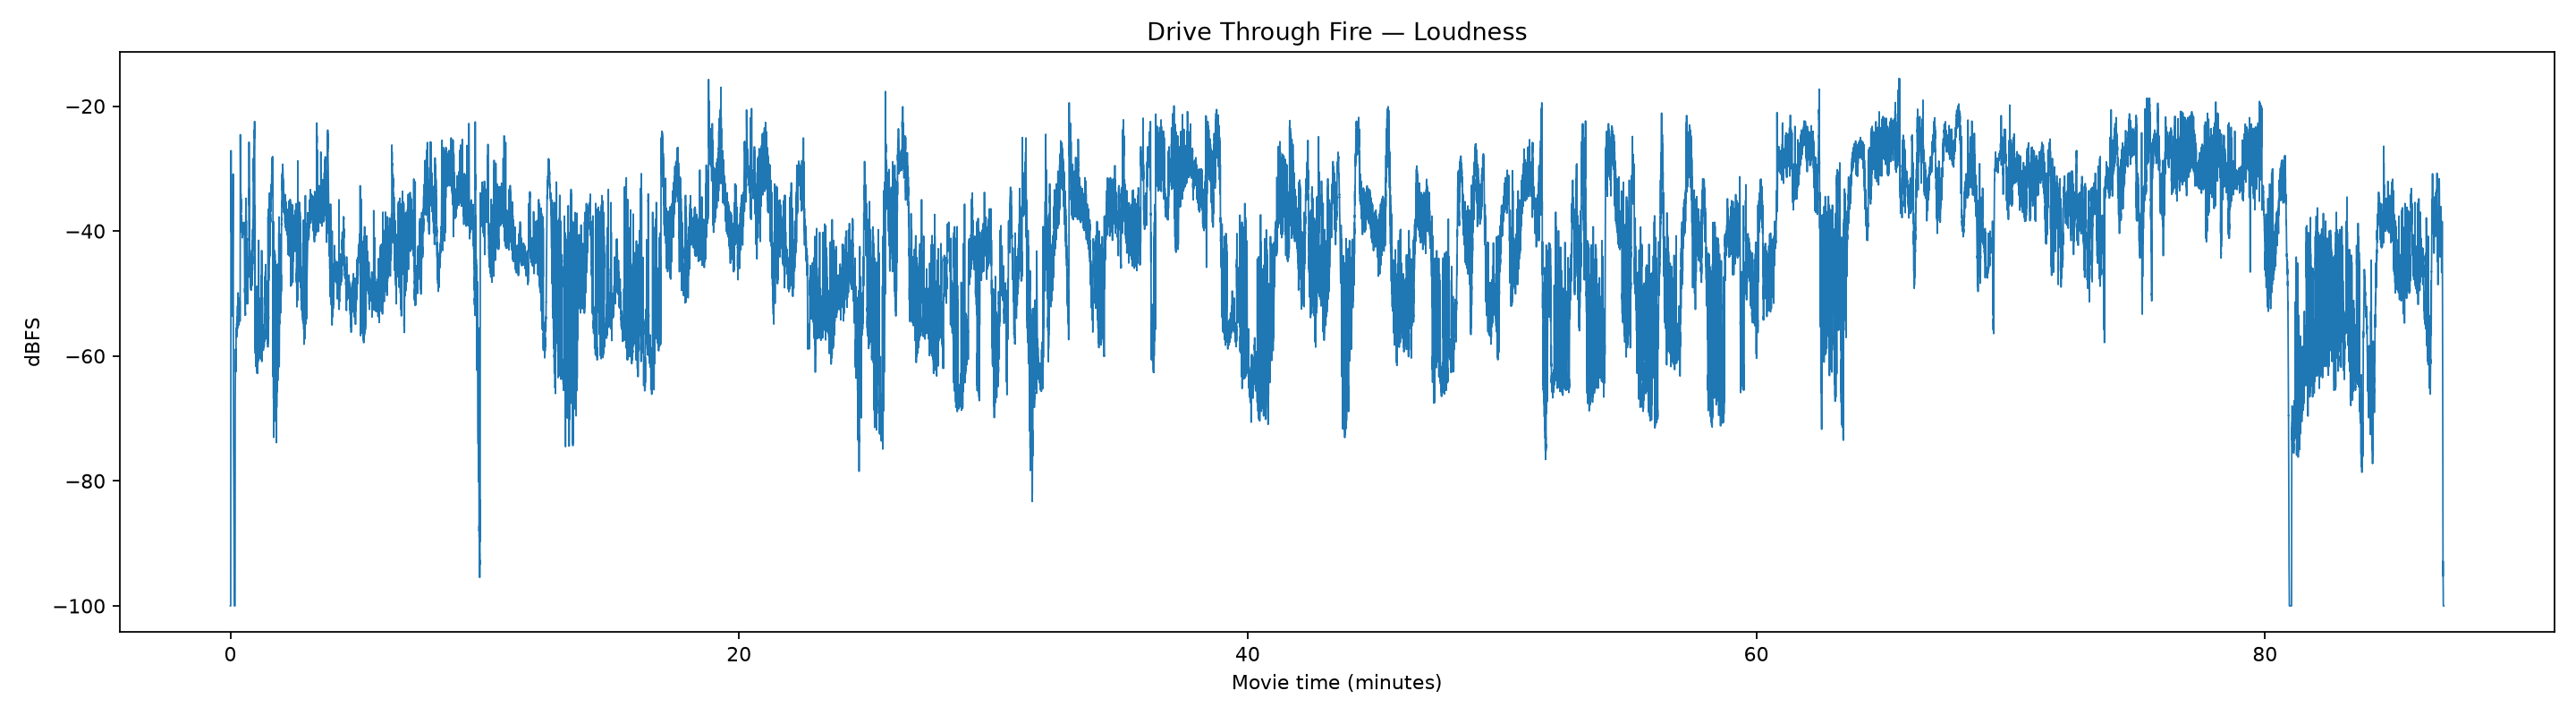
\includegraphics[width=\linewidth]{v3-01-loudness.png}
\caption{Version~3 harshness (top) and level (bottom). The three largest harshness spikes coincide with dropouts to $-100$~dBFS.}
\label{fig:harshfail}
\end{figure}

The same level invariance affected every onset-based measure. Between about 81 and 84 minutes the level trace sits mostly between $-55$ and $-75$~dBFS, far below the rest of the film, yet transient, barrage, low-frequency, and burden scores all peak there. An early reading of the plots described that stretch as the most intense passage of the film. It was a quiet passage with dense low-level transients. The subtitle timings introduced later (Chapter~\ref{ch:case}) identify it as the film's closing dialogue scene: more than half of its seconds carry subtitled speech, and its median level lies about 10~dB below the film's dialogue reference. The end credits begin only after about 84 minutes.

A synthetic test made the magnitude of the problem concrete. A passage of short noise bursts at a mono level of about $-83$~dBFS received a mean version~3 barrage score of 87, against 26 for a passage of modulated speech-band noise at about $-50$~dBFS, and a higher burden (0.54 against 0.50). After audibility weighting (Chapter~\ref{ch:pipeline}) the quiet passage scored $-7$ on barrage and 0.00 on burden, and the harshness score in digital silence fell to zero.

\section{Statistics fixed by their thresholds}

Version~3.1 on the film reported, among other things, that barrage regions occupied 8.0\% of the running time, high-load regions 15.8\%, and recovery regions 19.2\%, and that recovery was therefore scarce. These numbers are largely determined before any audio is analysed. High load is defined as the top 20\% of the burden score, so about 20\% of frames exceed the threshold by construction; the 15.8\% is the part of that 20\% that falls in runs of four seconds or more. Recovery is the bottom 25\%, so about a quarter of the film is recovery by definition; 19.2\% is the part in runs of five seconds or more. Barrage is the top 15\% of its score, of which 8.0\% survives the three-second minimum. Similarly, the 902 impact candidates are peaks above the 98.5th percentile at least 0.75~s apart; a different percentile gives a different count.

What these statistics can legitimately show is the arrangement in time of each category: where the qualifying windows fall, and the distribution of run lengths and gaps. The longest interval with no relative recovery window, 694.7 seconds, is such a statistic, and it is informative about the location of the film's densest stretch. It cannot show how much recovery the film provides compared with other films, because a film that was relentless from beginning to end would still be one quarter ``recovery''. The dialogue-referenced definitions of Chapter~\ref{ch:framework} were introduced for this reason.

\section{Interpretive overreach}

The fourth failure was not in the code. An interpretive pass over the version~3 and~3.1 plots, produced with the assistance of a language model, made a series of claims that the analysis could not support: that the 81 to 84 minute stretch was the most intense in the film (it was quiet; see above); that the film's recovery was scarce (a threshold artefact); that the film ``has plenty of dynamic range'' (the analysis measured unweighted RMS of a mono downmix, not loudness range in the standard sense); that swells of 30 to 36~dB demonstrated dramatic musical rises (the detector at that point checked only the end level of a swell, so a large rise could begin in near silence and could be a scene transition); and that the low-frequency detector found drums (it measures low-band onset density from any source).

Each claim was plausible, fluent, and consistent with the listener's report, which is what made it dangerous. The general lesson is that agreement between an analysis and a prior impression is weak evidence that the analysis is right. The specific corrections are built into the pipeline and into the reporting rules of Chapter~\ref{ch:case}: swell events carry their start and end levels; low-frequency activity is named for what it measures; percentile-defined totals are not reported as findings; and the loudness range of the film is reported only as measured under BS.1770 and EBU Tech~3342 (Chapter~\ref{ch:case}).

\section{Rules adopted}

\begin{enumerate}
\item Name each detector for the quantity it measures, not for the source it is hoped to find.
\item Test each detector on a synthetic signal with known contents, and inspect its output on real data against at least one independent trace.
\item Weight level-invariant features by audibility before standardising them, and compute statistics over audible frames.
\item Treat any total produced by a percentile threshold as a description of the threshold unless it is compared across films with a common threshold.
\item Report the start and end levels of every rise.
\item Do not accept an interpretation because it agrees with the listening report.
\end{enumerate}

\chapter{The Reproduction Chain}
\label{ch:chain}

A soundtrack file is not what a listener hears. Between the file and the ear lie a decoder, a downmix, a volume control, an amplifier, a loudspeaker, and a room. Film sound analysis usually treats this chain as transparent or as the listener's problem. This chapter treats it as part of the object of study, because in the case at hand it is likely to have made a difficult mix considerably worse, and because the same is probably true, in milder forms, of much ordinary home viewing.

\section{The chain in the case}

The film was played on a desktop computer. The computer's front-panel headphone output was connected by a 3.5~mm cable to a small solid-state bass practice amplifier, an Orange Crush 25BX, which has a single 8-inch driver and no separate high-frequency driver. The listener controlled level with the computer's volume control, which sits before the amplifier's input stage.

Several properties of the chain are not known and are recorded as open variables:
\begin{itemize}
\item the media player, and therefore the downmix it applied to the 5.1 stream, including whether the LFE channel was included;
\item which amplifier input received the signal (instrument input or an auxiliary input, if present), and therefore whether both channels of the headphone output were summed or only one was used;
\item the amplifier's gain, equaliser, and master settings;
\item the listening distance and room.
\end{itemize}

\section{Four transformations}

\subsection{Channel reduction}

Six channels become one loudspeaker. A player downmixing to stereo typically places the centre channel in both left and right at reduced level, together with the corresponding surrounds. If the stereo output then feeds a mono instrument input through a standard two-conductor plug, only the left channel reaches the amplifier and the right output is shorted to ground. In that case content panned to the right is lost, and dialogue is heard only through its share of the left channel. If the input sums both channels, material that is out of phase between left and right partially cancels. Either way the spatial separation that a multichannel mix uses to keep dialogue distinct from effects is removed. Separation by direction, one of the means by which a mix keeps several layers intelligible at once, is unavailable.

\subsection{Band limitation}

A single 8-inch driver in a small cabinet reproduces little of the lowest octave and has limited high-frequency extension. The important consequence is not the missing sub-bass but the relative treatment of the speech-importance band. The Speech Intelligibility Index weights most heavily the region from roughly one to four kilohertz \citep{ansi1997}. A bass instrument amplifier is voiced for the range where bass guitar fundamentals and low harmonics lie and is not designed to reproduce consonant cues clearly. Effects and music with substantial energy between 100~Hz and 1~kHz (impacts, engines, drums, low brass) are reproduced strongly. The effect is to lower dialogue intelligibility at a given level while leaving much of the energy of action material intact.

\subsection{Level-dependent distortion}

An instrument input is designed for the output of a passive bass pickup. A computer headphone output at a high volume setting can exceed that input's clean range, and the loudest passages of a film mix are exactly the ones that will do so. The amplifier's preamplifier then clips on transients, adding harmonic distortion products that are not in the file. The loudspeaker can also reach its excursion limit on strong low-frequency content. Both effects scale with level, so they concentrate where exceedance is already largest. Part of what a listener hears as harshness in such passages may be produced by the chain.\footnote{This is a mechanism, graded as hypothesised. It predicts that measured distortion in the chain's output rises sharply above a particular input level, and that recordings of the chain playing the film's loudest passages contain harmonic content absent from the source. Both predictions can be tested without rewatching the film.}

\subsection{Coupling of volume and distortion}

Because the listener's volume control precedes the amplifier, turning the volume down reduces both reproduced level and preamplifier drive. A reduction therefore relieves two problems at once. This is relevant to Chapter~\ref{ch:response}: in this chain, a logged volume reduction is a response to the combined effect of level and distortion, and the two cannot be separated behaviourally without the measurements below.

\section{How the chain enlarges exceedance}

Combining these transformations with the listener model of Chapter~\ref{ch:framework} gives a specific prediction. Let $D_{\text{file}}$ be the dialogue reference measured on the file and $D_{\text{heard}}$ the level at which the listener must set the chain for dialogue to be intelligible through it. Band limitation and channel reduction make intelligibility harder, so $D_{\text{heard}}$ is set higher relative to the file than it would be on a neutral system. Action material, reproduced strongly and with added distortion, then exceeds that higher setting by at least as much as before, and the effective exceedance
\begin{equation}
E_{\text{heard}}(t) = L_{\text{heard}}(t) - D_{\text{heard}}
\end{equation}
is at least as large as the file-level $E(t)$ and plausibly larger. The chain does not create the gap between dialogue and action, which is a property of the mix. It widens the gap and adds distortion to the loud side of it. This is the precise content of the observation that the amplifier ``exaggerated the bad mix''.

\section{Measuring the chain}

The chain can be characterised without watching the film again.

\begin{enumerate}
\item \textbf{Record the configuration.} Player and its audio output settings, the amplifier input used, all amplifier control positions, the computer volume setting, the cable, and the listening position.
\item \textbf{Frequency and impulse response.} Play an exponential sine sweep through the chain and record it at the listening position. Deconvolution yields the linear impulse response and separates harmonic distortion products in time \citep{farina2000}. A measurement microphone is preferable; a phone gives an approximate curve.
\item \textbf{Clipping onset.} Repeat the sweep at stepped computer volume settings and find the setting at which distortion products rise sharply.
\item \textbf{Absolute calibration.} Play a reference tone at a known digital level and read the sound pressure level at the seat with a meter. This converts dBFS in the file to dB SPL at the listener, and allows recovery windows and tolerances to be expressed in absolute rather than film-relative terms.
\item \textbf{Excerpt recordings.} Record the chain playing the audition clips (Chapter~\ref{ch:pipeline}) at the volume setting normally used, and compare each recording with its source.
\end{enumerate}

\section{Simulating the chain}

With an impulse response and a clipping model, the heard signal can be approximated from the file: apply the player's downmix, apply the listener's gain, apply a static nonlinearity with the measured onset, and convolve with the measured impulse response (\texttt{ffmpeg}'s \texttt{afir} filter performs the convolution). Running the pipeline of Chapter~\ref{ch:pipeline} on the simulated signal and on the file gives two sets of occupation measures for the same film. Their difference is a measurement of what the chain adds. Until that is done, statements about the chain in this book are graded as hypothesised.


\part{The Case}
\chapter{Case Study: \emph{Drive Through Fire}}
\label{ch:case}

\section{The film}

\emph{Drive Through Fire} is an action thriller directed by Lauren Bond and Jim Carlson, with Carlson and Michael Jai White in leading roles, released to video on demand and digital platforms on 11 September 2026 \citep{comingsoon2026}. Its published synopsis promises escalating violence ending in a rescue mission and a final confrontation, which is to say a genre in which extended gunfire and fight sequences are expected. Nothing in this chapter is a judgement of the film as a work. The question is how its soundtrack is organised in time relative to its dialogue, and what that organisation does to a listener at home.

The analysed file carries a six-channel 5.1 stream at 48~kHz. The decoded analysis stems run for 1:27:01.98, yielding 163{,}188 analysis frames.

\section{The listening report}

The report on which the case rests was given after a single viewing through the chain described in Chapter~\ref{ch:chain}. It makes four claims.

\begin{description}
\item[R1.] Dialogue was mixed lower than the sound effects, the swelling music, and the drums, and the difference was large enough to be comic.
\item[R2.] There were very long sequences of automatic gunfire and fighting.
\item[R3.] During those sequences the volume was reduced repeatedly, and in some cases turned fully off for one to two minutes or more, until the action on screen subsided.
\item[R4.] The amplifier exaggerated the imbalance.
\end{description}

The report is retrospective and has no timestamps. It is the observation that the rest of the book tries to explain and to make testable, not evidence for the framework. R1 and R2 are claims about the soundtrack and can be checked against the file. R3 is a claim about behaviour; the file can show whether the conditions the framework associates with such behaviour are present, but not that they caused it. R4 is a claim about the chain and is addressed only by the protocol of Chapter~\ref{ch:chain}.

\section{Descriptive output of the pipeline}

Table~\ref{tab:v31} gives the summary produced by version~3.1. Following the rules of Chapter~\ref{ch:failures}, its totals are reported as descriptions of the detectors at their thresholds, not as findings about the film.

\begin{table}[htbp]\centering\small
\begin{tabular}{lrl}
\toprule
Quantity & Value & Status \\
\midrule
Frames below audibility floor ($-65$ dBFS) & 3.2\% & measured \\
Impact candidates & 902 & threshold-determined \\
Low-frequency onset candidates & 52 & threshold-determined \\
Swell events & 78 & measured (event criteria) \\
Harshness candidates & 366 & threshold-determined \\
Barrage regions (time share) & 54 (8.0\%) & threshold-determined \\
High-load regions (time share) & 77 (15.8\%) & threshold-determined \\
Relative recovery regions (time share) & 78 (19.2\%) & threshold-determined \\
Median interval without relative recovery & 17.2 s & arrangement \\
Longest interval without relative recovery & 694.7 s & arrangement \\
\bottomrule
\end{tabular}
\caption{Version 3.1 summary for the film. ``Arrangement'' marks statistics that describe where threshold-defined events fall in time, which is informative within the film even though the totals are not.}\label{tab:v31}
\end{table}

Two arrangement statistics carry information. The median interval between relative recovery windows is 17.2 seconds: over most of the film, the soundtrack returns to its own quieter states frequently. The longest interval is 694.7 seconds, more than eleven and a half minutes. The distribution is therefore strongly skewed. Recovery is ordinarily frequent, and then for one long stretch it is absent.

\section{The shape of the film}

The version~3 traces, read with the caveats of Chapter~\ref{ch:failures}, show the arrangement that the skewed gap distribution implies. For the first hour the level trace alternates between passages near $-40$ to $-60$~dBFS and shorter excursions toward $-25$, with frequent relative recovery windows. From about 61 minutes the level rises and stays high, mostly between $-20$ and $-40$~dBFS, until about 80 minutes. On the version~3 recovery plot (Figure~\ref{fig:v3rec}) the relative recovery windows thin out after about 33 minutes and are almost absent between about 69 and 80 minutes. Low-frequency onset activity recurs throughout the film rather than being confined to its climax, with concentrations near 13 to 16, 38 to 45, 58 to 64, and 71 to 83 minutes.

\begin{figure}[htbp]\centering
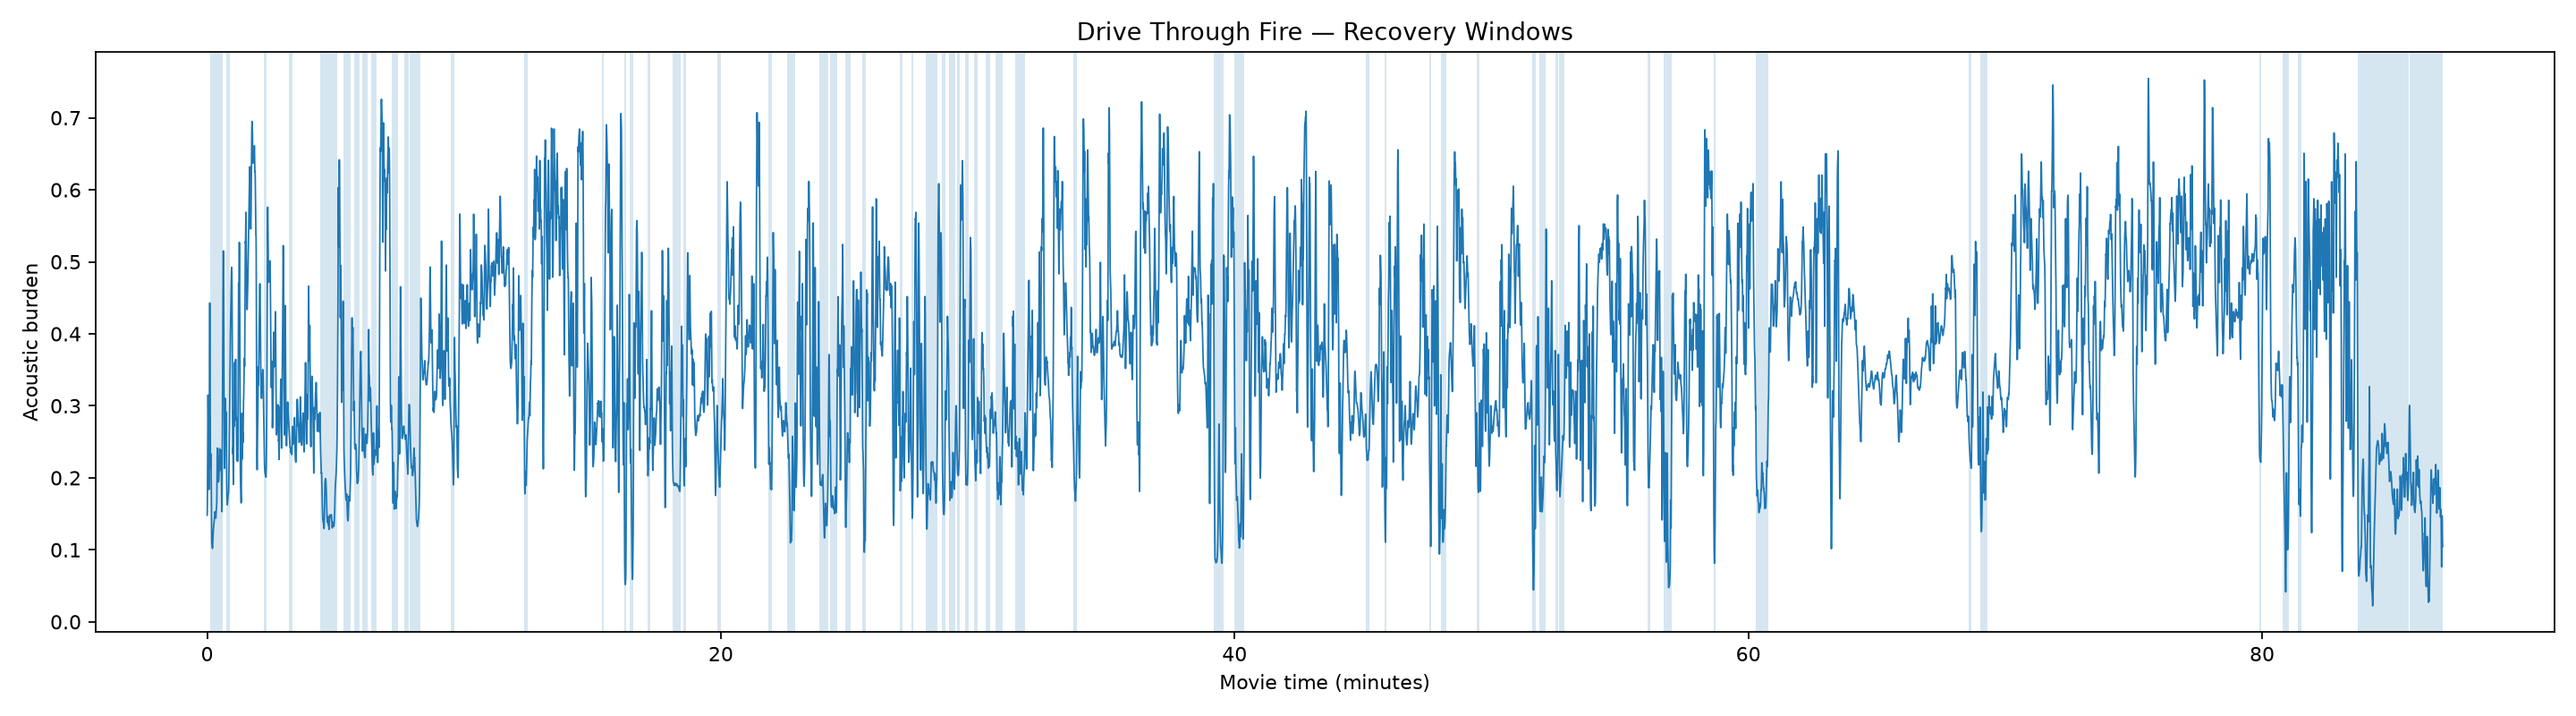
\includegraphics[width=\linewidth]{v3-09-recovery.png}
\caption{Version~3 burden with relative recovery windows shaded. The windows are frequent early, sparse after about 33 minutes, and nearly absent between about 69 and 80 minutes. Burden here is not audibility-weighted; the shaded region after about 84 minutes is the end credits.}
\label{fig:v3rec}
\end{figure}

% NOTE: numbers written as macros (\res..., \x...) are regenerated by
% code/occupation.py and code/occupation-extras.py. A few descriptive
% statements in this section (block times, segment percentages in the
% prose, the six-second agreement of gap locations) were written from the
% September 2026 run and must be re-checked if the analysis is rerun.
\section{Dialogue-referenced measures}

The measures of Chapter~\ref{ch:framework} were computed by \texttt{occupation.py} from the version~3.1 frame table, the film's 5.1 stream, and its subtitle file. \ifresults{Level is \resLevelMeasure, in \resLevelUnit.}{In this build the script has not been run, and every value below prints as \pending; Appendix~\ref{app:repro} gives the command.}

\subsection{Loudness by the standard measures}

By BS.1770 the film's integrated loudness is \resIntegrated~LUFS and its loudness range under EBU Tech~3342 is \resLRA~LU, spanning \resLRALow{} to \resLRAHigh~LUFS. These are the numbers a loudness-compliance check would report. They are given first because the rest of this section describes what they leave out: where in the film the loud material sits relative to the dialogue, and how long it stays there. Two relations are worth noting in advance. The dialogue reference found below lies \xDialogueBelowIntegrated~dB below the integrated loudness, so a playback system that normalised this film to a loudness target would place its dialogue that far below the target. And the upper bound of the loudness range, \resLRAHigh~LUFS, sits almost exactly where the plateau of loud material described below tops out.

\subsection{Subtitles and the dialogue proxy}

The subtitle file contains \resSubCues{} cues, of which \resSubNonspeechCues{} describe sound rather than speech and were removed, leaving \resSubSpeechCues. The applied offset is \resSubOffset~s; the correlation between cue coverage and centre-channel dominance is \resSubCorrZero{} with no shift and \resSubCorrOffset{} at the applied offset. After alignment, \resSubSeconds{} audible seconds are subtitled dialogue. No cue consisted solely of a sound description, so the file is an ordinary subtitle track rather than one written for deaf and hard-of-hearing viewers, and the best lag was zero: the subtitles were already aligned with this release.

Against these seconds, the centre-channel proxy (\resProxySeconds{} seconds) has a precision of \resProxyPrecision{} and a recall of \resProxyRecall. Precision measures how often the proxy's dialogue seconds are in fact subtitled speech; recall measures how much subtitled speech the proxy finds. The dialogue reference computed from the proxy is \resDialogueRefProxy~\resLevelUnit, against \resDialogueRefSub~\resLevelUnit{} from subtitles, and \resDialogueRefSubCapped~\resLevelUnit{} from subtitles with the most transient-heavy quarter removed. The three agree within about one decibel, so the results that follow do not depend on which definition of dialogue is used.

The combination is instructive. The proxy identifies dialogue seconds poorly, with precision and recall both near one half, yet it estimates dialogue \emph{level} almost exactly. Its errors are of two kinds that cancel in the median: centre-dominant seconds between cues (pauses, reactions, centre-panned ambience) that are at dialogue level without being subtitled, and subtitled seconds excluded by the transient cap or by a momentary loss of centre dominance. For a comparison corpus this is useful: films without subtitles can be given a dialogue reference from the proxy with some confidence, but not a dialogue timeline. The film's dialogue is strongly centred: the median centre advantage is \xCenterAdvDlg~dB in subtitled seconds against \xCenterAdvOther~dB elsewhere, which is the property the intervention of Chapter~\ref{ch:intervention} relies on.

\subsection{The dialogue reference}

The reference used below is taken from \resDialogueSource: $D = \resDialogueRef$~\resLevelUnit, computed from \resDialogueSeconds{} seconds (\resDialogueShare{} of the running time). The median centre-channel level in those seconds is \resDialogueCenter~dBFS. The reference is a median, and dialogue itself spans a wide range around it: the 10th and 90th percentiles of subtitled seconds lie at \xDlgPTen{} and \xDlgPNinety~dB relative to $D$, the quartiles at \xDlgPTwentyFive{} and \xDlgPSeventyFive~dB. Some of that spread is the dialogue and some is whatever else plays in the same second; the per-second level is the level of the whole mix. A listener anchored to dialogue is anchored to a band, not a line. \ifdefstring{\resDialogueFallback}{yes}{Fewer than thirty dialogue seconds were found, so the reference has fallen back to the median level of all audible seconds; in this build it should not be read as a dialogue level.}{}

\subsection{Exceedance}

Table~\ref{tab:exceed} gives the share of audible seconds whose level exceeds the dialogue reference by 5, 10, 15, and 20~dB, and Figure~\ref{fig:exceed} their distribution. The 95th percentile of exceedance is \resPNinetyFive~dB and the 99th is \resPNinetyNine~dB.

\begin{table}[htbp]\centering\small
\begin{tabular}{lr}
\toprule
Exceedance over dialogue reference & Share of audible seconds \\
\midrule
$\ge 5$ dB & \resExceedFive \\
$\ge 10$ dB & \resExceedTen \\
$\ge 15$ dB & \resExceedFifteen \\
$\ge 20$ dB & \resExceedTwenty \\
\bottomrule
\end{tabular}
\caption{Exceedance over the dialogue reference.}\label{tab:exceed}
\end{table}

\optfig{results/fig-exceedance.png}{0.7}{Distribution of per-second level relative to the dialogue reference. Blue: the reference. Red: the occupation tolerance $\delta = \resDelta$ dB.\label{fig:exceed}}

These figures bear on R1. A mix in which dialogue sits comfortably within the range of the rest of the soundtrack would show little mass beyond $+10$~dB. The size of that mass, and of the tail beyond $+20$~dB, measures how far a dialogue-anchored listening level is exceeded and how often. Set beside the loudness range above, they show the difference between the two kinds of description: loudness range reports how widely the level varies, while the exceedance distribution reports how far the level varies \emph{above the one level the listener cares about}.

For this film the answer is specific. Almost a third of the audible running time (\resExceedTen) lies at least 10~dB above the dialogue reference, but only \resExceedTwenty{} lies 20~dB or more above it. The occupied range is a plateau rather than a tail: among occupied seconds the median exceedance is \xOccMedian~dB, the 90th percentile \xOccPNinety~dB, and \xOccPlateauShare{} fall between $+12$ and $+19$~dB, after which the distribution falls away steeply (Figure~\ref{fig:exceed}). The loudest second in the film is \xLevelMax~LUFS, \xRelMax~dB above the reference. By peak intensity this is not an extreme soundtrack. What distinguishes it is how much time it spends in one band well above its dialogue. That is the distinction between peak intensity and occupation drawn in Chapter~\ref{ch:intro}, found in the data.\footnote{A plateau with a steep upper edge is what one would expect if loud material were held under a ceiling by compression or limiting in the mix or master. That is a hypothesis about production, not a measurement; the file shows the shape, not how it was made.}

\subsection{Occupation blocks}

With tolerance $\delta = \resDelta$~dB, merge gap $g = \resMergeGap$~s, and minimum length $m = \resMinBlock$~s, the analysis finds \resOccBlocksN{} occupation blocks, totalling \resOccTotalMin{} minutes. The longest lasts \resOccLongestMin{} minutes and begins at \resOccLongestStart. Table~\ref{tab:blocks} lists them with the implied throttle depth of Chapter~\ref{ch:framework}, the attenuation a listener who had set the volume for dialogue would need to hold each block's 95th-percentile level at tolerance. Across blocks the median implied throttle is \resThrottleMedian~dB and the largest is \resThrottleMax~dB.

Three blocks fall in the first hour, at about 8, 20, and 36 minutes, each isolated. The other six fall between 1:00:48 and 1:19:53. The last two are separated by only eleven seconds, so that from 1:13:45 to 1:19:53 the soundtrack is effectively a single block of about six minutes. Blocks do not contain all occupied time: of \xOccSeconds{} occupied seconds, \xOccInBlocks{} (\xOccInBlocksShare) fall in blocks and the rest in shorter episodes.

\begin{table}[htbp]\centering\small
\begin{tabular}{llrrrrr}
\toprule
Start & End & Min. & Median $E$ & $Q_{95}(E)$ & Throttle (dB) & Subtitled s \\
\midrule
\resOccRows \\
\bottomrule
\end{tabular}
\caption{Level-defined occupation blocks of at least \resMinBlock{} s. The last column counts subtitled dialogue seconds inside each block.}\label{tab:blocks}
\end{table}

\optfig{results/fig-occupation.png}{1.0}{Per-second level with the dialogue reference, the occupation tolerance, and occupation blocks shaded. Ticks along the bottom mark subtitled dialogue seconds.\label{fig:occ}}

An independent, transient-defined count comes from merging version~3.1 barrage regions across gaps of up to \resMergeGap~s. That procedure yields \resBarrageBlocksN{} blocks of at least \resMinBlock~s, the longest lasting \resBarrageLongestMin{} minutes. Figure~\ref{fig:blocks} compares the two definitions on a common time axis. Agreement between the two definitions would have been evidence that the blocks are properties of the soundtrack rather than of either detector. They do not agree. No merged barrage run reaches \resMinBlock~s; transient-defined episodes are scattered through the film and short. Inside level-defined blocks the mean barrage score is higher than outside (\xBarrageIn{} against \xBarrageOut) and the mean low-frequency onset score much higher (\xDrumIn{} against \xDrumOut), but neither forms continuous runs above the detectors' thresholds. The blocks are sustained in level; their onset density is episodic within them. Part of the disagreement is built into the barrage detector, whose percentile threshold and three-second minimum fragment long episodes. The rest is plausibly real: bursts of gunfire or impacts over a continuous loud bed of music and effects would produce exactly this pattern. The audition clips can decide between these readings.

\optfig{results/fig-blocks.png}{1.0}{Level-defined (top) and transient-defined (bottom) blocks. Dark segments meet the minimum length.\label{fig:blocks}}

\subsection{Two regimes}

The distribution of blocks and gaps suggests that the film changes character in its last half hour. Table~\ref{tab:segments} and Figure~\ref{fig:segments} make this explicit with fixed ten-minute segments, which involve no choice of boundary. For the first hour, between 13\% and 40\% of each segment lies 10~dB or more above dialogue and between 30\% and 51\% at or below it. In the two segments from 1:00:00 to 1:20:00 the proportions invert: 62\% and 71\% above, 14\% and 3\% at or below. The last segment, containing the closing dialogue scene and the credits, returns to the pattern of the first hour.

\begin{table}[htbp]\centering\small
\begin{tabular}{lrrrrr}
\toprule
Segment & $\ge +\delta$ (\%) & $\le D$ (\%) & In blocks (\%) & Subtitled (\%) & Median $E$ \\
\midrule
\xSegmentRows \\
\bottomrule
\end{tabular}
\caption{Ten-minute segments: share of audible seconds at least $\delta$ above the dialogue reference, at or below it, inside occupation blocks, and carrying subtitled speech, with median exceedance in dB.}\label{tab:segments}
\end{table}

\optfig{results/fig-segments.png}{0.95}{Share of audible seconds at least $\delta$ above the dialogue reference, at or below it, and carrying subtitled speech, by ten-minute segment.\label{fig:segments}}

The span defined by the longest recovery gaps and the two brief windows between them runs from \xSpanStart{} to \xSpanEnd, \xSpanMin{} minutes. Within it, \xSpanExceedShare{} of seconds lie at least $\delta$ above dialogue, \xSpanAtOrBelowShare{} at or below it, the median exceedance is \xSpanMedianRel~dB, and \xSpanInBlockShare{} of seconds belong to occupation blocks. The soundtrack returns to dialogue level for five seconds or more on only two occasions, totalling \xSpanRecoverySeconds{} seconds. Before \xSpanStart, the corresponding figures are \xBeforeExceedShare{} above, \xBeforeAtOrBelowShare{} at or below, and \xBeforeInBlockShare{} in blocks.

These results bear on R2 and R3. The framework predicts that fully turning the volume down for a minute or more occurs in blocks that are both long and deep, that is, with large implied throttle. The report is consistent with the framework if the film contains blocks of that kind. It would count against the framework's account of the report if the film contained no such blocks: if, for example, exceedances were large but brief, or long but shallow.

\subsection{Dialogue exposed to throttling}

Occupation blocks are not free of speech. Across all blocks, \resSubInBlocks{} subtitled dialogue seconds fall inside them, \resSubInBlocksShare{} of all subtitled dialogue in the film; the block from 1:09:24 to 1:11:34 alone contains 48. The median level of these seconds is \xDlgInBlockMedian~dB relative to the reference, against \xDlgOutBlockMedian~dB for subtitled seconds outside blocks. Because the per-second level is that of the whole mix, this does not say the speech is loud; it says the speech occurs inside the loud material. Whether it remains intelligible there is a question of masking, which this analysis does not measure. This is the dialogue a listener loses by turning the volume down or off for the duration of a block, and it quantifies the dilemma of Chapter~\ref{ch:intro}: in these seconds the soundtrack asks to be heard and to be turned down at the same time. The subtitles also give the listener a partial remedy, which is to read what cannot be heard; that the remedy exists at all is a measure of the problem.

\subsection{Recovery}

Using the absolute definition (at least five seconds at or below the dialogue reference, or inaudible), the film contains \resAbsRecoveryN{} recovery windows, covering \resAbsRecoveryShare{} of its running time. The longest gap between them lasts \resAbsGapLongestMin{} minutes and begins at \resAbsGapLongestStart. The maximum recovery debt accumulated within a single gap is \resDebtMax~dB$\cdot$s. The longest relative-recovery gap from Table~\ref{tab:v31} lasts \resRecoveryGapLongestMin{} minutes and begins at \resRecoveryGapLongestStart. The two definitions, one based on the film's own quietest quarter and the other on its dialogue level, place their longest gaps within six seconds of each other. The location of the film's longest stretch without rest does not depend on how rest is defined. A recovery gap is not an occupation block: a gap measures how long the soundtrack goes without returning to dialogue level, while a block measures how long it stays at least $\delta$ above it. A long gap may contain a block, several short ones, or none.

\begin{table}[htbp]\centering\small
\begin{tabular}{llr}
\toprule
Gap start & Gap end & Minutes \\
\midrule
\resAbsGapRows \\
\bottomrule
\end{tabular}
\caption{The five longest gaps between absolute recovery windows.}\label{tab:gaps}
\end{table}

\subsection{Swells}

The swell detector found \resSwellN{} sustained rises, of which \resSwellLarge{} rise by 20~dB or more. Only \resSwellFromQuiet{} begin below \resSwellQuietLevel~\resLevelUnit, near the audibility floor, where a large rise is more likely to be an entry from near silence or a scene transition than a crescendo. The concern raised in Chapter~\ref{ch:failures}, that large detected rises might mostly be entries from silence, therefore does not hold for this film: most begin from audible levels. \resSwellIntoOcc{} of the \resSwellN{} end in the occupied range, at or above $D+\delta$. These are the swells that matter for the listener model, rises that carry the soundtrack from a level set for dialogue into the range where the volume must come down. Whether they are musical is a question for the audition clips.

\section{Assessment}

\begin{description}
\item[R1] is borne out by the file. Measured against its own subtitled dialogue, the film spends \resExceedTen{} of its audible running time at least 10~dB above dialogue level and \resExceedFifteen{} at least 15~dB above it, while its dialogue is strongly centred and its loud material is held on a plateau 12 to 19~dB above the reference. Whether this makes the dialogue ``mixed too low'' or the effects ``mixed too high'' is the same measurement described two ways.
\item[R2] is borne out in level and not in onset density. The film contains \resOccBlocksN{} blocks of a minute or more at least 10~dB above dialogue, six of them in its last half hour and one effectively six minutes long. The transient detectors do not find sustained barrages of comparable length; onset activity is elevated but episodic within the blocks.
\item[R3] cannot be tested against the file, but the conditions the framework associates with turning the volume fully down are present: long blocks with implied throttle depths from \xThrottleMin{} to \resThrottleMax~dB (median \resThrottleMedian~dB), and a span of \xSpanMin{} minutes in which the soundtrack returns to dialogue level for only \xSpanRecoverySeconds{} seconds. The reported behaviour, turning the volume off for one to two minutes or more, matches the lengths of the blocks in that span.
\item[R4] remains untested.
\end{description}

The case therefore supports the central distinction of the book at the grade ``measured'': this soundtrack is not distinguished by extreme peaks but by the amount and continuity of time it spends in one band well above its dialogue, concentrated in a single twenty-minute stretch with almost no return to rest.

\chapter{Overdetermination}
\label{ch:overdetermination}

Level is not the only way a soundtrack claims attention. An abrupt onset claims it; so does a rhythmic low-frequency pulse, a rising swell, and bright, noisy spectral content. This chapter considers what happens when several of these channels are used at once, and what the present measurements can and cannot say about it.

\section{The idea}

A single moment in an action sequence may contain a physical impact, a vocal cry, a percussive hit in the score, a rising orchestral or synthetic swell, and the broadband noise of breaking glass or gunfire. Each layer, taken alone, is ordinary craft. Murch's account of density describes how layers are distributed so that each remains legible \citep{murch2005}, and Chion's notion of added value describes how sound directs the interpretation of the image \citep{chion1994}. The concern here is different. When several channels are elevated together, they may be communicating the same thing, an instruction to attend now, through redundant means. The word \emph{overdetermination} is used for this: an effect produced by more causes than are needed to produce it.

Redundancy is not in itself a defect; it makes a signal robust. The hypothesis of Chapter~\ref{ch:framework} is narrower. It is that, at a given level of exceedance, a moment in which more salience channels are elevated is more likely to provoke a volume reduction, and that sustained overdetermination contributes to the listener's sense that the soundtrack never stops demanding attention.

\section{Measurement}

The overdetermination index $\Omega(t)$ counts, for each second, how many of five channels are elevated: level exceedance ($E\ge\delta$), transient barrage, low-frequency onset activity, harshness, and an active swell event. Channels other than exceedance count as elevated when their per-second score exceeds 1.5 on the pipeline's standardised scale.

Because several channels share components with level (see below), the index is also computed in a residualised form, $\Omega_{\text{res}}$. For each channel, a quadratic in $L(t)$ is fitted across audible seconds, and the channel counts as elevated only if it exceeds the raw threshold \emph{and} at least half that margin remains after the level-predicted value is subtracted. By construction $\Omega_{\text{res}}\le\Omega$.

\begin{table}[htbp]\centering\small
\begin{tabular}{lrr}
\toprule
 & $\Omega$ & $\Omega_{\text{res}}$ \\
\midrule
Mean within occupation blocks & \resOmegaIn & \resOmegaResIn \\
Mean outside occupation blocks & \resOmegaOut & \resOmegaResOut \\
Share of audible seconds with $\ge 3$ channels & \resOmegaThreeShare & \resOmegaResThreeShare \\
Share of block seconds with $\ge 3$ channels & \resOmegaThreeShareIn & \resOmegaResThreeShareIn \\
\bottomrule
\end{tabular}
\caption{Overdetermination, raw and residualised on level.}\label{tab:omega}
\end{table}

The difference between the two columns estimates how much of the apparent co-elevation is mechanical. What remains in the residualised column is co-elevation that level does not explain.

\section{Result for the case}

At first sight the index doubles inside occupation blocks, raw and residualised alike. But one of its five channels is exceedance itself, which is present in nearly every block second by definition. Removing that term leaves the number of \emph{other} channels elevated per second: \xOtherRawIn{} inside blocks against \xOtherRawOut{} outside on the raw scale, and \xOtherResIn{} against \xOtherResOut{} after residualising on level. The doubling is carried entirely by exceedance. Excluding it, the blocks are no more overdetermined than the rest of the film, and after removal of the level dependence slightly less so. Seconds with three or more channels elevated are rare everywhere: \resOmegaResThreeShare{} of audible seconds and \resOmegaResThreeShareIn{} of block seconds on the residualised index.

The channel means tell the same story with one qualification. Low-frequency onset activity is much higher on average inside blocks (\xDrumIn{} against \xDrumOut), and barrage somewhat higher (\xBarrageIn{} against \xBarrageOut), while harshness is about the same (\xHarshIn{} against \xHarshOut). These elevations are mostly below the channel threshold. The blocks carry more low-frequency rhythmic activity, but not in a way that stacks with the other channels.

For this film, at these thresholds, the soundtrack-side premise of the overdetermination hypothesis is not supported. What distinguishes its occupied stretches is sustained level, with somewhat denser low-frequency activity, not a pile-up of independent salience channels.

\section{What the index cannot show yet}

Three limitations prevent these numbers from testing the hypothesis.

First, the channels are not independent by construction. The barrage and harshness scores each include a level term, and every onset-based measure is audibility-weighted by level. A rise in level therefore raises several channels mechanically. The residualised index addresses the part of this coupling that a smooth function of level can capture.\footnote{Residualising on a quadratic in level removes the average dependence of each channel on level, not every interaction. A channel whose relation to level differs between scenes (for example, harshness that rises with level in gunfire but not in music) is only partly corrected.}

Second, the channels are acoustic, not semantic. Elevated low-frequency onset activity may be a drum, an engine, or a sequence of impacts. The overdetermination hypothesis is about distinct sources carrying the same message, which requires knowing what the sources are. The audition clips exist for this purpose, and Chapter~\ref{ch:response} describes how their annotation should be conducted.

Third, the hypothesis is about behaviour. Co-elevation is only interesting if it predicts volume reductions beyond what exceedance predicts, and that requires the response data specified in the next chapter.

\section{A note on the earlier reading}

Version~3's plots appeared to show every channel rising together between about 81 and 84 minutes, and an early reading took this as the clearest instance of overdetermination in the film. Chapter~\ref{ch:failures} showed that this stretch was quiet and that its apparent intensity was an artefact of level-invariant features. The episode is a warning specific to this chapter's subject: an index that counts coincident elevations will find the most coincidences wherever a shared artefact touches every channel at once. Audibility weighting removes the artefact that produced that particular coincidence. Residualising on level removes much of the mechanical coupling that remains.

\section{Status}

Overdetermination is graded as hypothesised. For this film the index finds no excess co-elevation in occupation blocks once exceedance itself is set aside. That result is limited by the acoustic channels chosen and their thresholds, and it says nothing yet about sources or behaviour: a scream, a gunshot, and a drum hit in the same second could all register in one channel. The hypothesis is therefore weakened rather than rejected. Source labels from the blinded annotation are the next test of it.


\part{Response and Intervention}
\chapter{The Hand on the Volume}
\label{ch:response}

The framework's hypotheses are about behaviour: when listeners reduce the volume, how far, and for how long. This chapter specifies how that behaviour can be recorded and how a study should be designed so that the resulting data can confirm or refute the framework rather than decorate it.

\section{Origin of the measure}

The idea of treating volume behaviour as data predates this analysis. A set of design notes from July 2025, kept in the author's public repository, proposed a tool provisionally called MuteNet: a background process that records when viewers mute, when they drop the volume sharply, and when they restore it after a loud scene, and that aggregates these records across viewers to identify consensus moments of unpleasant sound and to train models of them \citep{flyxion2025}. The same notes proposed the intervention developed in Chapter~\ref{ch:intervention}. The present chapter turns the first proposal into a measurement protocol.

\section{Why volume behaviour}

Volume behaviour has three advantages as a dependent variable. It is produced during viewing rather than recalled afterwards. It is continuous in time and can be aligned exactly with the soundtrack. And, as the noise-control literature suggests \citep{glass1972}, it is a direct expression of the listener exercising control over the sound, which is the phenomenon at issue. Its disadvantage is that it confounds several motives (level, distortion, content, fatigue, and the wish to hear the next line of dialogue), which is why it must be combined with the chain measurements of Chapter~\ref{ch:chain} and the annotations described below.

\section{Recording}

The script \texttt{throttle-log.lua} (Appendix~\ref{app:code}) runs inside the \texttt{mpv} player and writes a record each time the volume, mute state, or pause state changes, stamped with the film time, the wall-clock time, the slider value, and the corresponding gain in decibels. A key binding records a marker when something bothers the viewer without a volume change. The protocol requires that system volume and amplifier settings be fixed and recorded before viewing and that the viewer adjust level only within the player, so that the logged gain is the only gain that changes.

From the log the following variables are derived:
\begin{description}
\item[Reduction onset.] A time at which gain decreases by at least 3~dB within two seconds.
\item[Reduction depth.] The gain change in dB, with full muting or a slider at zero treated as a separate outcome, \emph{off}.
\item[Listener recovery time.] The time from a reduction until gain returns to within 3~dB of its prior value.
\item[Marker.] A timestamp without gain change.
\end{description}

Listener recovery time is the behavioural counterpart of the soundtrack's recovery windows. The comparison of the two is the most direct test the framework admits: whether listeners restore the volume when, and only when, the soundtrack returns to dialogue level.

\section{Annotation of candidates}

The audition clips produced by the pipeline allow the acoustic detectors to be tied to identified sources, but only under conditions that prevent the annotator's expectations from determining the labels.

\begin{enumerate}
\item \textbf{Blind presentation.} Clips are renamed with random identifiers and shuffled across categories. Detector name, score, and timestamp are withheld until labelling is complete.
\item \textbf{Random controls.} Thirty to fifty windows drawn uniformly from the audible portion of the film are mixed in with the detector clips. Without them, the proportion of detector clips labelled as unpleasant has no baseline and cannot show that the detectors select anything.
\item \textbf{Several dimensions.} Each clip receives a source label from a fixed vocabulary (Appendix~\ref{app:instrument}), a role (voice, music, effect, ambience, mixed), an intensity rating from one to five, and a binary judgement of whether the listener would reduce the volume.
\item \textbf{More than one listener.} Three to five listeners allow inter-rater agreement to be computed and turn the single-listener limitation into a measurement of variation between listeners.
\end{enumerate}

The pipeline's annotation summary then reports, for each detector, the share of its clips that were not false positives and the distribution of source labels, which can be compared with the same distribution for the random controls.

\section{Design}

\subsection{Pre-registration}

Before any response data are examined, the predictions of Chapter~\ref{ch:framework} are to be written down with their direction and the variables that operationalise them. The listening report was produced before the analysis. The analysis has since been seen by the listener, and any further viewing of this film by the same listener is a repeat viewing informed by the plots. That contamination is unavoidable for this listener and film and must be stated; it is avoidable for new listeners and new films.

\subsection{Comparison corpus}

A single film cannot show that its occupation is unusual. A corpus of five to ten films, including films of the same genre from earlier decades and films of other genres from the same period, analysed with a common dialogue-referenced method and thresholds fixed across the corpus, would allow the case's exceedance and block statistics to be placed in a distribution. The percentile-based detectors of the current pipeline would need pooled thresholds for this purpose.

\subsection{Playback conditions}

Each listener should view under at least two conditions: the chain of interest and a neutral reference (headphones or monitors of known response), with order counterbalanced across listeners and films. This separates what listeners respond to in the mix from what they respond to in the chain, which is the objection a reviewer would raise first to any single-chain study.

\section{Analysis}

The primary model is a discrete-time hazard model. For each second in which the listener has not already reduced the volume, the outcome is whether a reduction onset occurs in that second. Predictors are current exceedance $E(t)$; time already elapsed in the current occupation block; recovery debt $K(t)$; the residualised overdetermination index; the playback condition; and listener and film random effects. The hypotheses of Chapter~\ref{ch:framework} map onto coefficients: occupation over level (block elapsed time and $E$ outperform instantaneous level alone, and whole-film statistics add nothing), recovery debt (positive coefficient on $K$), overdetermination (positive coefficient on $\Omega$ at fixed $E$), and chain amplification (positive effect of the chain condition, larger at high $E$).

A secondary model predicts listener recovery time from the time until the soundtrack's next absolute recovery window. A tertiary analysis predicts the \emph{off} outcome specifically from block length and implied throttle depth.

\section{Aggregation}

The MuteNet proposal envisaged aggregation across many viewers. The log format above is sufficient for that purpose and contains nothing about the viewer beyond their volume behaviour and the film's identity. Aggregated over viewers, reduction onsets form an empirical annoyance curve for a film, which could be published alongside it much as loudness metadata already is, and which would give sound designers a direct view of where home listeners reach for the control.

\chapter{Remixing for the Listener}
\label{ch:intervention}

A listener who reduces the volume during an action sequence is already remixing the film, crudely, with a single global gain. This chapter considers how that remix can be done less crudely, beginning with what is possible now on any 5.1 source and ending with more speculative tools.

\section{A continuum of interventions}

The July 2025 notes that proposed the response measure of Chapter~\ref{ch:response} also proposed a pair of tools, a ``whisperizer'' and a ``mufflerizer'' \citep{flyxion2025}. In their most radical form they would re-render all dialogue as whispered speech, detect gunshots, explosions, and screams, remove them, replace each class with a stylised musical substitute, and signal the substitution visually on screen. Taken literally this is a transformation of the film into a different work. Taken as the far end of a continuum, it clarifies the design space:

\begin{enumerate}
\item \textbf{Global gain.} The listener's volume control. Available everywhere; sacrifices dialogue to control action or the reverse.
\item \textbf{Global dynamic range control.} Consumer ``night mode'' and decoder compression profiles. Reduces the gap between loud and quiet without regard to source.
\item \textbf{Channel-based rebalancing.} Raising the channel that carries most dialogue relative to the others, then compressing. Available on any discrete multichannel source.
\item \textbf{Separated rebalancing.} Estimating a dialogue stem by source separation, for sources in which dialogue is not isolated by channel, and rebalancing it against the rest.
\item \textbf{Class-specific attenuation.} Detecting particular event classes and attenuating them selectively.
\item \textbf{Class-specific substitution.} Replacing detected classes with other sounds and, optionally, visual cues.
\end{enumerate}

\section{A dialogue-forward downmix}

Level 3 is available today with \texttt{ffmpeg} or with the \texttt{mpv} player, which accepts \texttt{ffmpeg} filters during playback. The following plays a 5.1 film with the centre channel forward, everything else reduced, the result compressed and limited, and the output in mono:

\begin{lstlisting}[language=bash,numbers=none]
mpv --af="lavfi=[pan=mono|c0=1.0*FC+0.35*FL+0.35*FR+0.25*SL+0.25*SR,acompressor=threshold=-24dB:ratio=6:attack=5:release=250:makeup=6dB,alimiter=limit=-3dB]" film.mkv
\end{lstlisting}

The same filter chain in an \texttt{ffmpeg} command renders a permanently rebalanced copy of the file:

\begin{lstlisting}[language=bash,numbers=none]
ffmpeg -i film.mkv -map 0:v -map 0:a:0 -c:v copy \
  -af "pan=mono|c0=1.0*FC+0.35*FL+0.35*FR+0.25*SL+0.25*SR,acompressor=threshold=-24dB:ratio=6:attack=5:release=250:makeup=6dB,alimiter=limit=-3dB" \
  -c:a aac -b:a 160k film-dialogue-forward.mkv
\end{lstlisting}

Each stage has a purpose. The \texttt{pan} stage reweights channels before they are summed, raising dialogue relative to effects and music by roughly 9 to 12~dB compared with an equal-weight sum, and produces a single channel so that a mono chain receives the whole mix regardless of which conductor its plug connects. The compressor reduces the level of passages above its threshold by a factor of six, with a fast attack to catch impacts and a moderate release to avoid audible pumping between lines, and restores overall level with make-up gain. The limiter enforces a ceiling so that transients the compressor misses cannot drive a downstream preamplifier into clipping. The weights and time constants are starting points, tested for correct operation on a synthetic multichannel file, and are meant to be adjusted by ear.

\section{Limitations}

Channel-based rebalancing inherits the limits of the dialogue proxy of Chapter~\ref{ch:framework}. Effects panned to the centre are raised with the dialogue; dialogue spread into the front pair is partly lowered with the effects. Compression changes the character of the mix everywhere, not only where it is needed. And on stereo sources there is no centre channel to raise, which is where level 4 becomes necessary.

\section{Beyond channels}

Levels 4 to 6 depend on models. Neural source separation can estimate a dialogue stem from a stereo mix, and sound event detection models trained on large labelled corpora \citep{gemmeke2017} can mark gunshots, explosions, and screams in time. Next-generation broadcast audio formats already carry dialogue as a separate object with user-adjustable level, which makes level 4 a matter of metadata rather than estimation for programmes delivered in those formats. Class-specific substitution (level 6) is a creative transformation rather than a correction; it has an accessibility rationale for viewers with sound sensitivity, for whom certain classes of sound are the barrier to watching at all, and a clear risk of misclassification, which is a reason to signal substitutions visibly rather than silently.

\section{The objection from intent}

An intervention of any of these kinds alters what the filmmakers made. The objection deserves a direct answer. The dynamic relationships of a film mix are authored for a calibrated room (Chapter~\ref{ch:background}). In an uncalibrated home, through an arbitrary chain, those relationships are already not reproduced, and the listener already intervenes with the volume control, in the crudest possible way and at the cost of whole scenes of dialogue. The choice is not between the authored mix and an altered one. It is between an alteration performed by hand, reactively, with one global control, and an alteration designed to keep the dialogue the film depends on while bringing the rest into a range the room can carry.

\section{Evaluation}

Hypothesis~5 of Chapter~\ref{ch:framework} states what the intervention must achieve: fewer and shorter volume reductions without loss of dialogue comprehension. The design of Chapter~\ref{ch:response} tests it directly by adding the rebalanced mix as a playback condition, with comprehension assessed by brief questions on dialogue content after each viewing. An intervention that reduces throttling by making dialogue as hard to follow as the action is not a success.


\part{Conclusion}
\chapter{What Has Been Shown}
\label{ch:conclusion}

\section{The argument in brief}

The difficulty of watching certain films at home is usually described as a matter of loudness. This monograph has argued that the better description is occupation: the extent to which a soundtrack stays far above the level its dialogue requires, and for how long it does so without returning. Standard loudness measures summarise distributions and cannot see this temporal property. A listener anchored to dialogue meets it directly, as a sequence of exceedances to be managed by hand, and a long, deep block of exceedance leaves only one practical response, which is to turn the sound off and wait.

\section{Graded claims}

Table~\ref{tab:grades} collects the principal claims of the book with their grades.

\begin{longtable}{p{0.62\linewidth}lc}
\toprule
Claim & Grade & Chapter \\
\midrule
\endhead
Integrated loudness and loudness range are distributional and do not describe the temporal arrangement of exceedances & Established & \ref{ch:background} \\
Cinema reproduction is calibrated to a reference level; home reproduction generally is not & Established & \ref{ch:background} \\
Perceived control over noise reduces its aftereffects & Established & \ref{ch:background} \\
Speech intelligibility depends most on roughly the one to four kilohertz region & Established & \ref{ch:background} \\
The default \texttt{ffmpeg} mono downmix of a tagged 5.1 stream omits the LFE channel & Measured & \ref{ch:pipeline} \\
The film's relative recovery windows are ordinarily frequent (median gap 17.2 s) but absent for one stretch of 694.7 s & Measured & \ref{ch:case} \\
The film's level is high and sustained from roughly 61 to 80 minutes & Measured & \ref{ch:case} \\
Low-frequency onset activity recurs throughout the film rather than only at its climax & Measured & \ref{ch:case} \\
The film's integrated loudness is \resIntegrated~LUFS and its loudness range \resLRA~LU & Measured & \ref{ch:case} \\
The dialogue reference lies \xDialogueBelowIntegrated~dB below integrated loudness & Measured & \ref{ch:case} \\
\resExceedTen{} of audible time lies at least 10~dB above subtitled dialogue level, but only \resExceedTwenty{} at least 20~dB above; loud material forms a plateau from about $+12$ to $+19$~dB & Measured & \ref{ch:case} \\
The film contains \resOccBlocksN{} occupation blocks of at least a minute, six of them after the first hour & Measured & \ref{ch:case} \\
From \xSpanStart{} to \xSpanEnd{} the soundtrack returns to dialogue level for only \xSpanRecoverySeconds~s & Measured & \ref{ch:case} \\
Relative and absolute definitions of recovery locate the longest gap in the same place & Measured & \ref{ch:case} \\
The loud plateau reflects compression or limiting in the mix or master & Hypothesised & \ref{ch:case} \\
\resSubInBlocksShare{} of subtitled dialogue falls inside occupation blocks & Measured & \ref{ch:case} \\
The centre-channel proxy locates dialogue poorly (precision and recall near one half) but estimates its level within about 1~dB & Measured & \ref{ch:case} \\
Excluding exceedance itself, occupation blocks are not more overdetermined than the rest of the film & Measured & \ref{ch:overdetermination} \\
Most large swells begin from audible levels rather than near silence & Measured & \ref{ch:case} \\
Level-defined occupation blocks coincide with sustained transient barrages & Rejected & \ref{ch:case} \\
Volume reductions are predicted by occupation variables better than by level or whole-film statistics (H1) & Hypothesised & \ref{ch:framework} \\
Reduction probability rises with recovery debt (H2) & Hypothesised & \ref{ch:framework} \\
Reduction probability rises with overdetermination at fixed exceedance (H3) & Hypothesised (premise weakened) & \ref{ch:overdetermination} \\
The bass-amplifier chain widened the dialogue-to-action gap and added distortion to loud passages (H4) & Hypothesised & \ref{ch:chain} \\
A dialogue-forward downmix reduces throttling without loss of comprehension (H5) & Hypothesised & \ref{ch:intervention} \\
Version 3 swell candidates identify swells & Rejected & \ref{ch:failures} \\
Version 3 harshness peaks identify harsh material & Rejected & \ref{ch:failures} \\
The stretch from 81 to 84 minutes is the most intense in the film (it is the quiet closing dialogue scene) & Rejected & \ref{ch:failures} \\
Percentile-defined totals show that the film's recovery is scarce & Rejected & \ref{ch:failures} \\
The early analysis had established that the film ``has plenty of dynamic range'' & Rejected & \ref{ch:failures} \\
Swell events of 30 dB or more are musical crescendos & Rejected (untested) & \ref{ch:failures} \\
The low-frequency detector identifies drums & Rejected & \ref{ch:failures} \\
\bottomrule
\caption{Principal claims and their grades.}\label{tab:grades}
\end{longtable}

\section{Limitations}

The study rests on one film, one listener, one viewing, and one unmeasured reproduction chain. Its dialogue reference depends on subtitle timing, which marks when speech occurs but not every utterance, and which may be imperfectly aligned with the analysed release. Its frame-level detectors, apart from the swell detector, still use unweighted features and film-internal percentile thresholds, even though the occupation measures now use BS.1770 loudness. Its residualised overdetermination index removes only the smooth dependence of each channel on level. Its response data consist of a retrospective report without timestamps. Each of these limitations has a remedy specified in the text: pooled thresholds across a corpus, psychoacoustic replacements for the spectral descriptors, source labels from blinded annotation, the logging protocol of Chapter~\ref{ch:response}, and the chain measurements of Chapter~\ref{ch:chain}.

\section{A programme}

The research programme that follows from the framework has five components, in order of cost:
\begin{enumerate}
\item characterise the reproduction chain with a sine sweep and a level calibration;
\item conduct blind, multi-listener annotation of the audition clips with random controls;
\item log volume behaviour for new viewings under at least two playback conditions, including the dialogue-forward downmix;
\item analyse a comparison corpus with common, dialogue-referenced thresholds;
\item fit the hazard models of Chapter~\ref{ch:response} and report which hypotheses survive.
\end{enumerate}

\section{Closing}

The instruments built for this study failed several times before they measured anything, and the failures were more convincing than the successes until they were checked. That history is part of the result. A complaint about a soundtrack is easy to confirm with plots that are drawn after the complaint is made. It is harder, and more useful, to specify in advance what the soundtrack would have to contain for the complaint to be explained, to measure whether it does, and to name the listener data that could show the explanation wrong. The concept of occupation is offered as the core of such a specification.


\appendix
\chapter{Reproducing the Results}
\label{app:repro}

The numerical results of Chapter~\ref{ch:case} are produced in two steps from the film file. The first step decodes the film and takes the longest; the second runs in seconds.

\begin{lstlisting}[language=bash,numbers=none]
# 1. Frame features, detector events, audition clips
python3 code/analyze-soundtrack-v3.1.py drive-through-fire-2026.mkv \
    --title "Drive Through Fire" --out sound-analysis-v3.1

#    (or, reusing an existing version 3 frame table)
python3 code/analyze-soundtrack-v3.1.py drive-through-fire-2026.mkv \
    --from-frames sound-analysis-v3/frames.csv --out sound-analysis-v3.1

# 2. Dialogue-referenced measures, figures, and LaTeX macros
python3 code/occupation.py \
    --frames sound-analysis-v3.1/frames.csv \
    --events sound-analysis-v3.1/events.csv \
    --film drive-through-fire-2026.mkv \
    --subtitles drive-through-fire-2026.srt \
    --out results

#    supplementary statistics and the segment figure
python3 code/occupation-extras.py --results results

# 3. Blinded annotation set with random controls (Chapter 9)
python3 code/blind-audition.py drive-through-fire-2026.mkv \
    --audition sound-analysis-v3.1/audition \
    --frames sound-analysis-v3.1/frames.csv --out blind --controls 40

# 4. Build the manuscript
pdflatex main.tex && pdflatex main.tex
\end{lstlisting}

Step~2 decodes the film once more to measure BS.1770 loudness (cached in \texttt{results/loudness.csv} for later runs), estimates the subtitle offset, and writes \texttt{results/results.tex}, which the manuscript reads at compile time, together with \texttt{fig-occupation.png}, \texttt{fig-exceedance.png}, \texttt{fig-blocks.png}, a per-second table \texttt{seconds.csv}, and \texttt{occupation.json}. If \texttt{results/results.tex} is absent, every dependent value prints as \pending.

Dependencies are \texttt{ffmpeg}, Python~3 with \texttt{numpy}, \texttt{scipy}, \texttt{pandas}, \texttt{matplotlib}, \texttt{soundfile}, and \texttt{librosa}, and a standard \LaTeX{} installation.

\chapter{Annotation Instrument}
\label{app:instrument}

\section{Label vocabulary}

Source labels, of which one or more may be assigned to a clip, joined with \texttt{+}:

\begin{center}\small
\begin{tabular}{llll}
DRUM & MUSIC\_SWELL & MUSIC\_OTHER & SIREN \\
ALARM & GUNSHOT & EXPLOSION & PUNCH \\
CRASH & GLASS & ENGINE & TIRES \\
YELLING & SCREAM & CROWD & DIALOGUE \\
FALSE\_POSITIVE & UNSURE & & \\
\end{tabular}
\end{center}

\section{Fields}

\begin{center}\small
\begin{tabularx}{\linewidth}{lX}
\toprule
Field & Content \\
\midrule
\texttt{clip} & Random identifier assigned at blinding \\
\texttt{label} & Source labels from the vocabulary \\
\texttt{role} & voice, music, effect, ambience, or mixed \\
\texttt{intensity} & 1 (barely noticeable) to 5 (overwhelming) \\
\texttt{would\_reduce} & yes or no: would the listener reduce the volume \\
\texttt{notes} & Free text \\
\bottomrule
\end{tabularx}
\end{center}

Detector category, score, film time, and whether the clip is a random control are held in a separate key file (\texttt{key.csv}, written by \texttt{blind-audition.py}) and joined to the labelled sheet on the \texttt{clip} column only after labelling is complete. Random control clips appear in the key with category \texttt{RANDOM\_CONTROL}.

\chapter{Code}
\label{app:code}

The four programs used in this study are reproduced in full. All are released into the public domain.

\section{Feature extraction and detection}
\lstinputlisting[language=Python]{code/analyze-soundtrack-v3.1.py}

\section{Dialogue-referenced occupation analysis}
\lstinputlisting[language=Python]{code/occupation.py}

\section{Supplementary statistics}
\lstinputlisting[language=Python]{code/occupation-extras.py}

\section{Blinded annotation set}
\lstinputlisting[language=Python]{code/blind-audition.py}

\section{Volume behaviour logger for \texttt{mpv}}
\lstinputlisting{code/throttle-log.lua}


\backmatter
\begin{thebibliography}{99}
\addcontentsline{toc}{chapter}{References}

\bibitem[ANSI(1997)]{ansi1997}
ANSI (1997). \emph{ANSI S3.5-1997: Methods for Calculation of the Speech Intelligibility Index}. American National Standards Institute, New York.

\bibitem[ATSC(2013)]{atsc85}
ATSC (2013). \emph{A/85: Techniques for Establishing and Maintaining Audio Loudness for Digital Television}. Advanced Television Systems Committee, Washington, DC.

\bibitem[ATSC(2018)]{atsc52}
ATSC (2018). \emph{A/52: Digital Audio Compression (AC-3, E-AC-3) Standard}. Advanced Television Systems Committee, Washington, DC.

\bibitem[Bello et~al.(2005)]{bello2005}
Bello, J.~P., Daudet, L., Abdallah, S., Duxbury, C., Davies, M., and Sandler, M.~B. (2005). A tutorial on onset detection in music signals. \emph{IEEE Transactions on Speech and Audio Processing}, 13(5), 1035--1047.

\bibitem[Bregman(1990)]{bregman1990}
Bregman, A.~S. (1990). \emph{Auditory Scene Analysis: The Perceptual Organization of Sound}. MIT Press, Cambridge, MA.

\bibitem[CALM Act(2010)]{calm2010}
Commercial Advertisement Loudness Mitigation Act (2010). Public Law 111--311, United States.

\bibitem[Chion(1994)]{chion1994}
Chion, M. (1994). \emph{Audio-Vision: Sound on Screen}. Edited and translated by C.~Gorbman. Columbia University Press, New York.

\bibitem[ComingSoon(2026)]{comingsoon2026}
ComingSoon.net (2026). Spawn's Michael Jai White gets his Liam Neeson \emph{Taken} moment in \emph{Drive Through Fire} trailer. August 2026. \url{https://www.comingsoon.net/?p=2181827}.

\bibitem[EBU(2016)]{ebu3342}
EBU (2016). \emph{Tech 3342: Loudness Range, A Measure to Supplement EBU R\,128 Loudness Normalisation}. European Broadcasting Union, Geneva.

\bibitem[EBU(2020)]{ebu128}
EBU (2020). \emph{R\,128: Loudness Normalisation and Permitted Maximum Level of Audio Signals}. European Broadcasting Union, Geneva.

\bibitem[Farina(2000)]{farina2000}
Farina, A. (2000). Simultaneous measurement of impulse response and distortion with a swept-sine technique. \emph{108th Convention of the Audio Engineering Society}, Paris.

\bibitem[Fastl and Zwicker(2007)]{fastl2007}
Fastl, H. and Zwicker, E. (2007). \emph{Psychoacoustics: Facts and Models}, 3rd ed. Springer, Berlin.

\bibitem[Flyxion(2025)]{flyxion2025}
Flyxion (2025). Pitch control per speaker (design notes, July 2025, including MuteNet and the whisperizer and mufflerizer proposals). \texttt{standardgalactic/kitbash}, file \texttt{workspace/Pitch control per speaker.txt}. \url{https://github.com/standardgalactic/kitbash}.

\bibitem[Gemmeke et~al.(2017)]{gemmeke2017}
Gemmeke, J.~F., Ellis, D.~P.~W., Freedman, D., Jansen, A., Lawrence, W., Moore, R.~C., Plakal, M., and Ritter, M. (2017). Audio Set: An ontology and human-labeled dataset for audio events. In \emph{Proceedings of IEEE ICASSP 2017}, 776--780.

\bibitem[Glass and Singer(1972)]{glass1972}
Glass, D.~C. and Singer, J.~E. (1972). \emph{Urban Stress: Experiments on Noise and Social Stressors}. Academic Press, New York.

\bibitem[Goodman(2010)]{goodman2010}
Goodman, S. (2010). \emph{Sonic Warfare: Sound, Affect, and the Ecology of Fear}. MIT Press, Cambridge, MA.

\bibitem[ITU-R(2015)]{itu1770}
ITU-R (2015). \emph{Recommendation BS.1770-4: Algorithms to Measure Audio Programme Loudness and True-Peak Audio Level}. International Telecommunication Union, Geneva.

\bibitem[Johnston(1988)]{johnston1988}
Johnston, J.~D. (1988). Transform coding of audio signals using perceptual noise criteria. \emph{IEEE Journal on Selected Areas in Communications}, 6(2), 314--323.

\bibitem[Kerins(2011)]{kerins2011}
Kerins, M. (2011). \emph{Beyond Dolby (Stereo): Cinema in the Digital Sound Age}. Indiana University Press, Bloomington.

\bibitem[Kryter(1985)]{kryter1985}
Kryter, K.~D. (1985). \emph{The Effects of Noise on Man}, 2nd ed. Academic Press, Orlando.

\bibitem[McFee et~al.(2015)]{mcfee2015}
McFee, B., Raffel, C., Liang, D., Ellis, D.~P.~W., McVicar, M., Battenberg, E., and Nieto, O. (2015). librosa: Audio and music signal analysis in Python. In \emph{Proceedings of the 14th Python in Science Conference}, 18--25.

\bibitem[Miedema and Oudshoorn(2001)]{miedema2001}
Miedema, H.~M.~E. and Oudshoorn, C.~G.~M. (2001). Annoyance from transportation noise: Relationships with exposure metrics DNL and DENL and their confidence intervals. \emph{Environmental Health Perspectives}, 109(4), 409--416.

\bibitem[Moore(2012)]{moore2012}
Moore, B.~C.~J. (2012). \emph{An Introduction to the Psychology of Hearing}, 6th ed. Emerald, Bingley.

\bibitem[Murch(2005)]{murch2005}
Murch, W. (2005). Dense clarity, clear density. \emph{The Transom Review}, 5(1).

\bibitem[Schafer(1977)]{schafer1977}
Schafer, R.~M. (1977). \emph{The Tuning of the World}. Knopf, New York.

\bibitem[Sergi(2004)]{sergi2004}
Sergi, G. (2004). \emph{The Dolby Era: Film Sound in Contemporary Hollywood}. Manchester University Press, Manchester.

\bibitem[SMPTE(2012)]{smpte200}
SMPTE (2012). \emph{RP 200: Relative and Absolute Sound Pressure Levels for Motion-Picture Multichannel Sound Systems}. Society of Motion Picture and Television Engineers, White Plains, NY.

\bibitem[Vickers(2010)]{vickers2010}
Vickers, E. (2010). The loudness war: Background, speculation, and recommendations. \emph{129th Convention of the Audio Engineering Society}, San Francisco.

\end{thebibliography}


\end{document}
